% =====================================================================
% Marco Práctico --- Sección 3.9: Etapa 4
% =====================================================================

\subsection{Etapa 4 --- Arquitecturas Matriciales y No Idealidades}
\label{ch:fase4}

La Etapa 4 estudia implementaciones a nivel de red mediante un
arreglo cruzado bidimensional (crossbar). Su aplicación al agente de
control se desarrolla en la subseccion siguiente. Los resultados
corresponden a modelos y entornos de simulación, no a mediciones de
un crossbar fabricado.

% =====================================================================
\subsubsection{Etapa 4.1: Matriz Crossbar e In-Memory}
\label{sec:etapa4_1}

Una matriz crossbar se representa por
$\mathbf{G}\in\mathbb{R}^{N\times M}$, con $N$ filas de entrada y
$M$ columnas de salida; cada intersección aloja un dispositivo
memristivo simulado.

En el modelo ideal, al aplicar un vector de voltajes de entrada
$\mathbf{V}=[V_1,V_2,\dots,V_N]^{\mathsf T}\in\mathbb{R}^{N}$ a las
filas, las conductancias en paralelo realizan una multiplicación
matriz-vector. La corriente $I_j$ de cada columna sigue la ley de Ohm
y la ley de corrientes de Kirchhoff:

\begin{equation}
I_j(t) = \sum_{i=1}^N V_i(t) \cdot G_{ij}(t) \quad \implies \quad \mathbf{I} = \mathbf{G}^{\mathsf T} \mathbf{V},\qquad \mathbf{I}\in\mathbb{R}^{M}
\label{eq:vmm_law}
\end{equation}

En un arreglo analógico ideal, las contribuciones de las celdas se procesarían en paralelo. Esta descripción algebraica no demuestra latencia física constante ni complejidad computacional $\mathcal{O}(1)$ para el solver numérico: el costo de resolver el modelo MNA se trata por separado en el Experimento~9.

\paragraph{Implementación Cualitativa (Operación Analógica $1 \times 1$)}
Se implementó y se visualizó estructuralmente el sistema base modular probando una celda atómica unitaria que simula la interacción macro-escalar. 

Como se ilustra en las salidas de simulación (Figuras~\ref{fig:crossbar_1x1_completo}a-d), al suministrar la onda cuadrada de voltaje al modelo, la dinámica de la celda memristiva de Yakopcic cambia su estado. La línea de columna calcula $\mathbf{I}=\mathbf{G}^{\mathsf T}\mathbf{V}$ en el modelo, con las filas de $\mathbf{G}$ asociadas a las entradas y las columnas a las salidas. Estas figuras ilustran la operación implementada; no son mediciones de hardware ni prueban por sí solas su comportamiento físico.

\begin{figure}[H]
    \centering
    \begin{subfigure}[b]{0.84\textwidth}
        \centering
        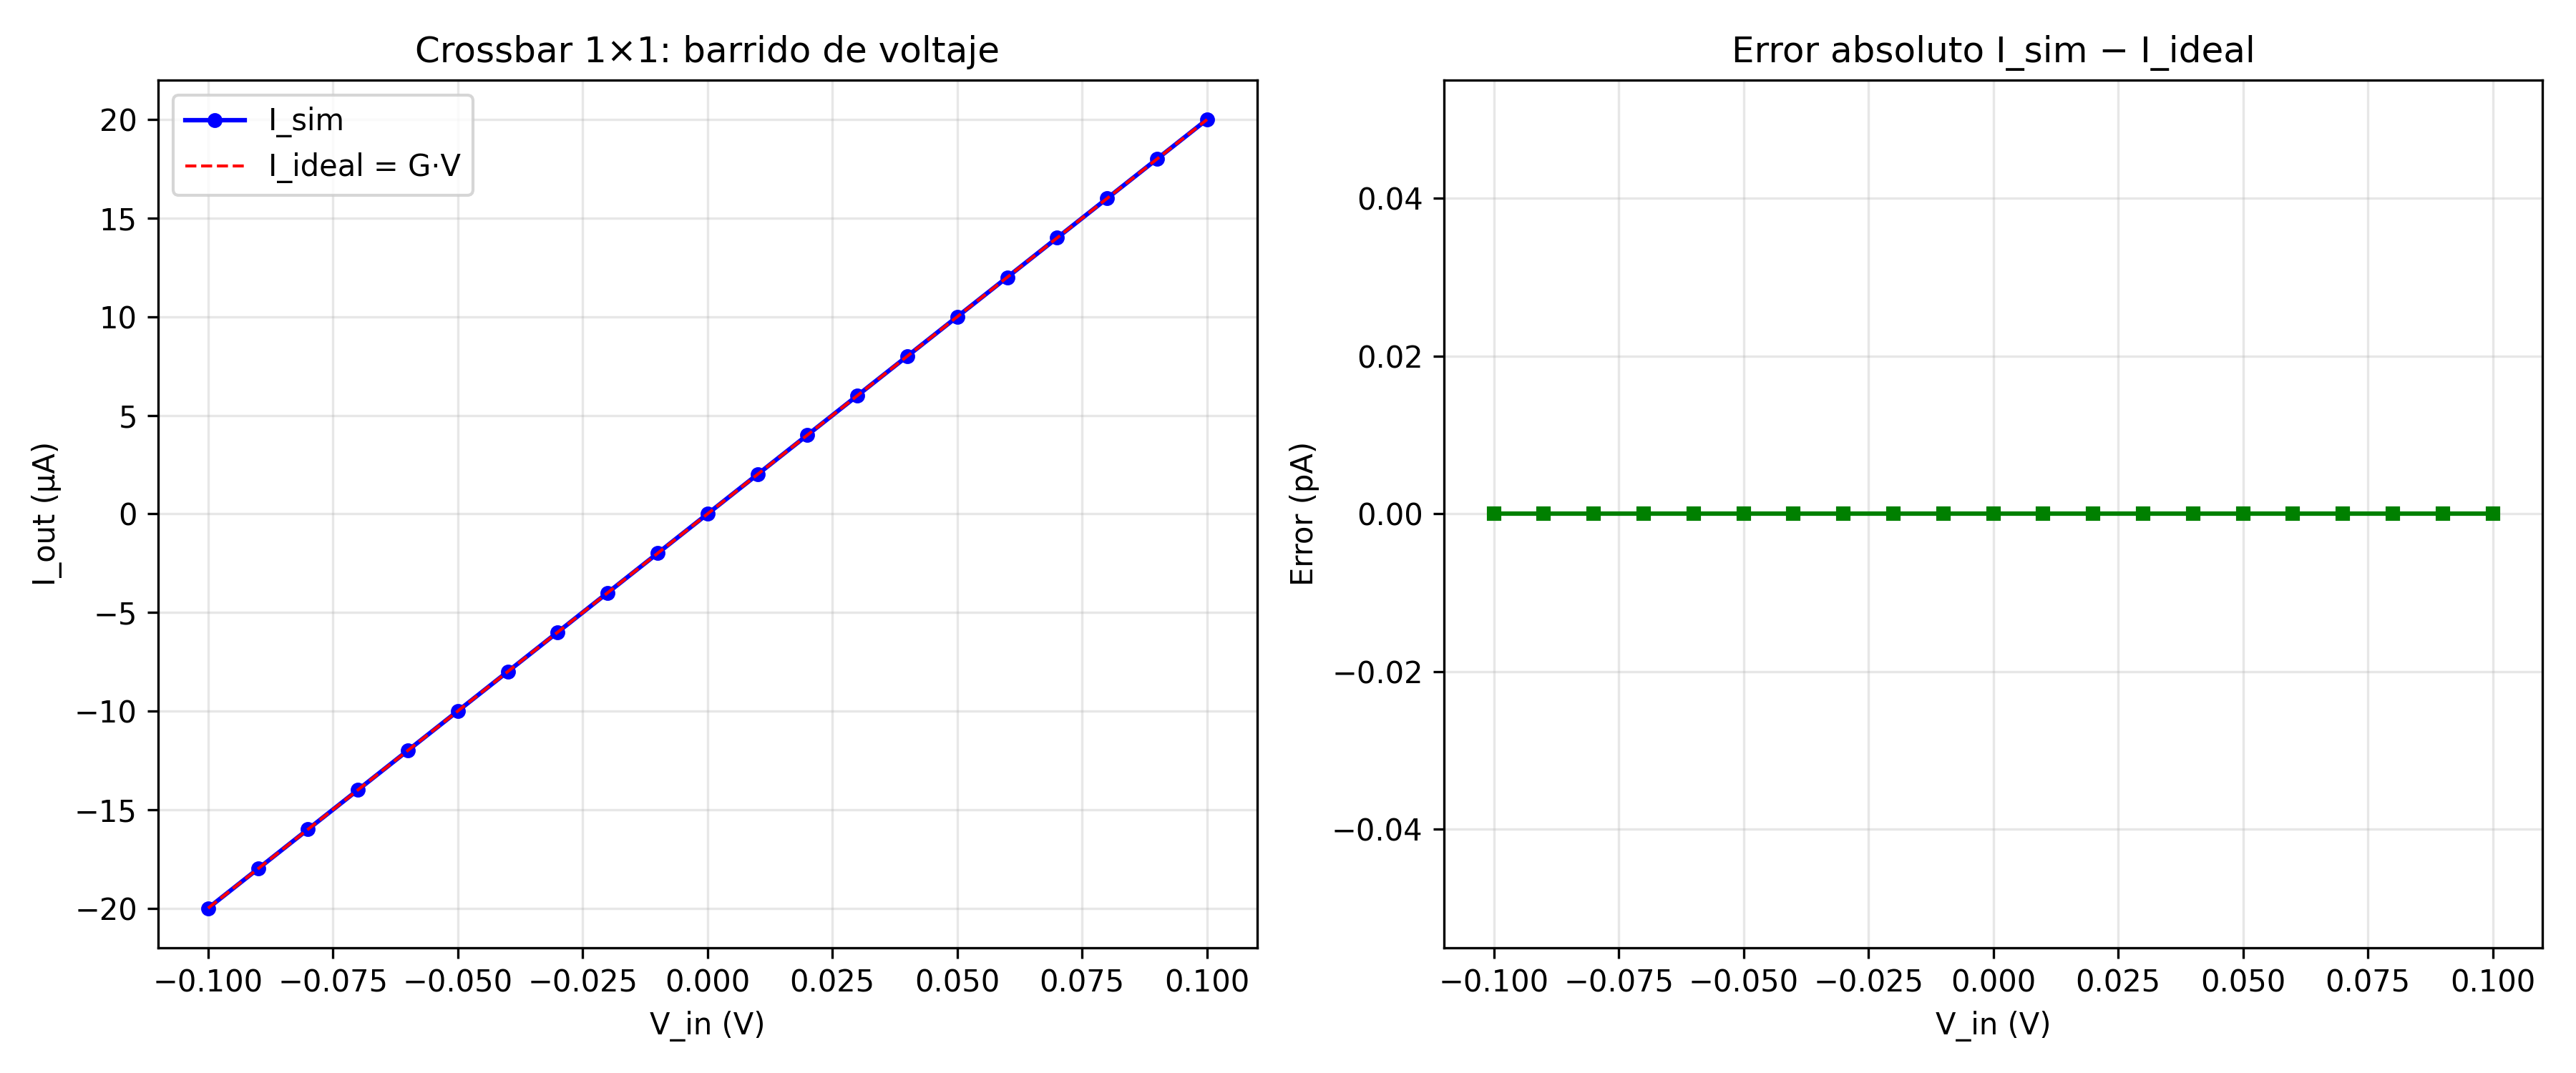
\includegraphics[width=\textwidth]{figuras/fig_21a_crossbar_V.png}
        \caption{Pulsos de excitación por línea de Palabra $V_i(t)$.}
    \end{subfigure}
    \vskip 0.3cm
    \begin{subfigure}[b]{0.84\textwidth}
        \centering
        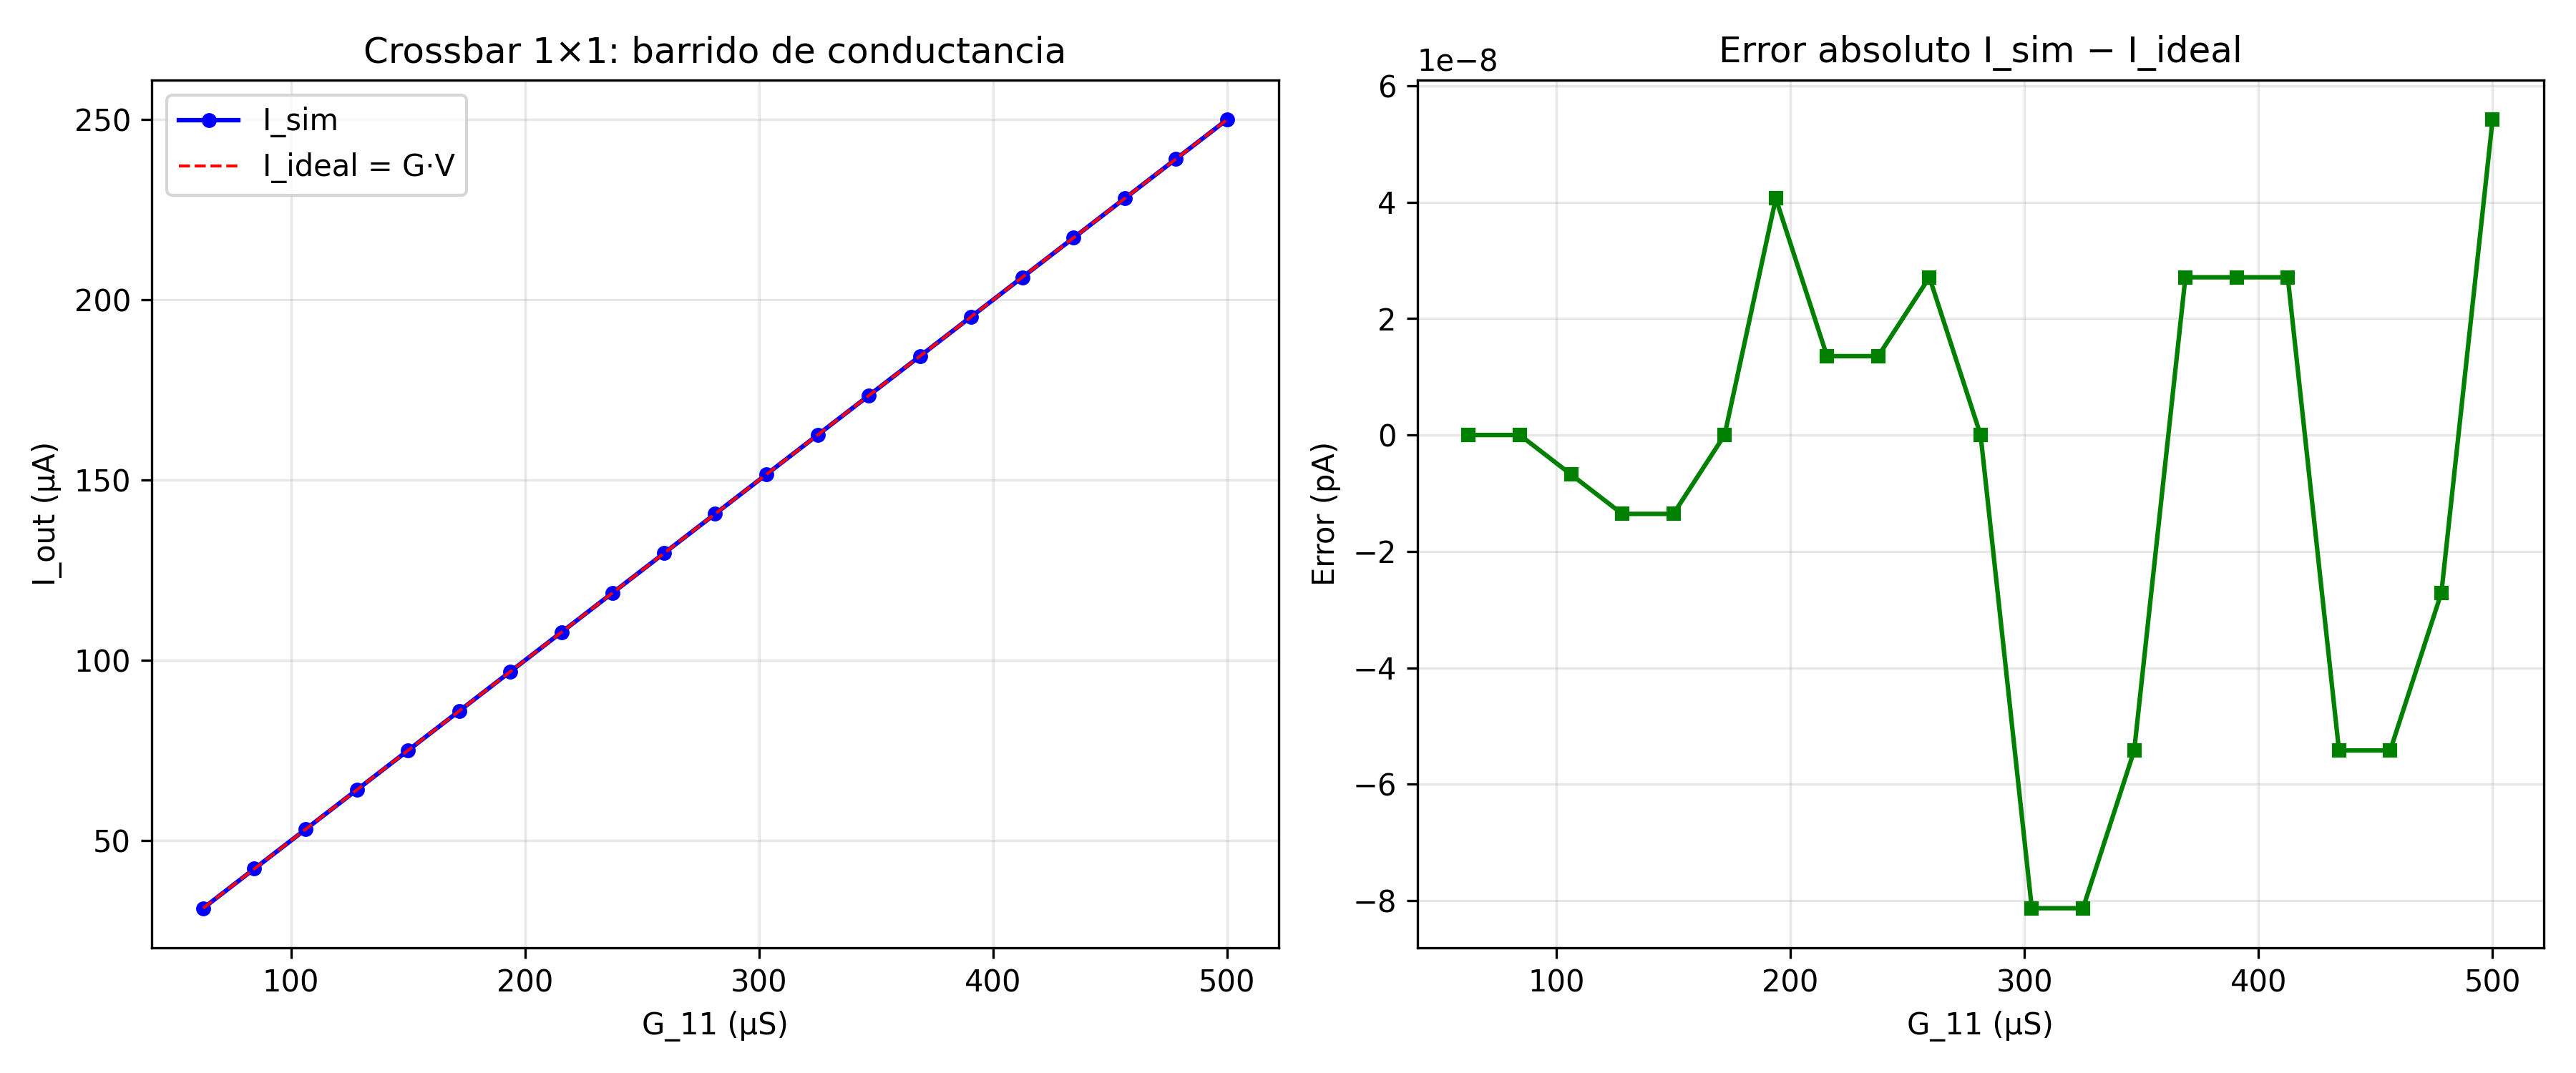
\includegraphics[width=\textwidth]{figuras/fig_21b_crossbar_G.png}
        \caption{Matriz espacial de conductancia transversal $G_{ij}(t)$.}
    \end{subfigure}
    \caption[Verificación funcional del crossbar analógico]{Verificación cualitativa y funcional de computación In-Memory en el bloque elemental Crossbar analógico (paneles a y b).}
    \label{fig:crossbar_1x1_completo}
\end{figure}

\clearpage

\begin{figure}[H]
    \ContinuedFloat
    \centering
    \begin{subfigure}[b]{0.84\textwidth}
        \centering
        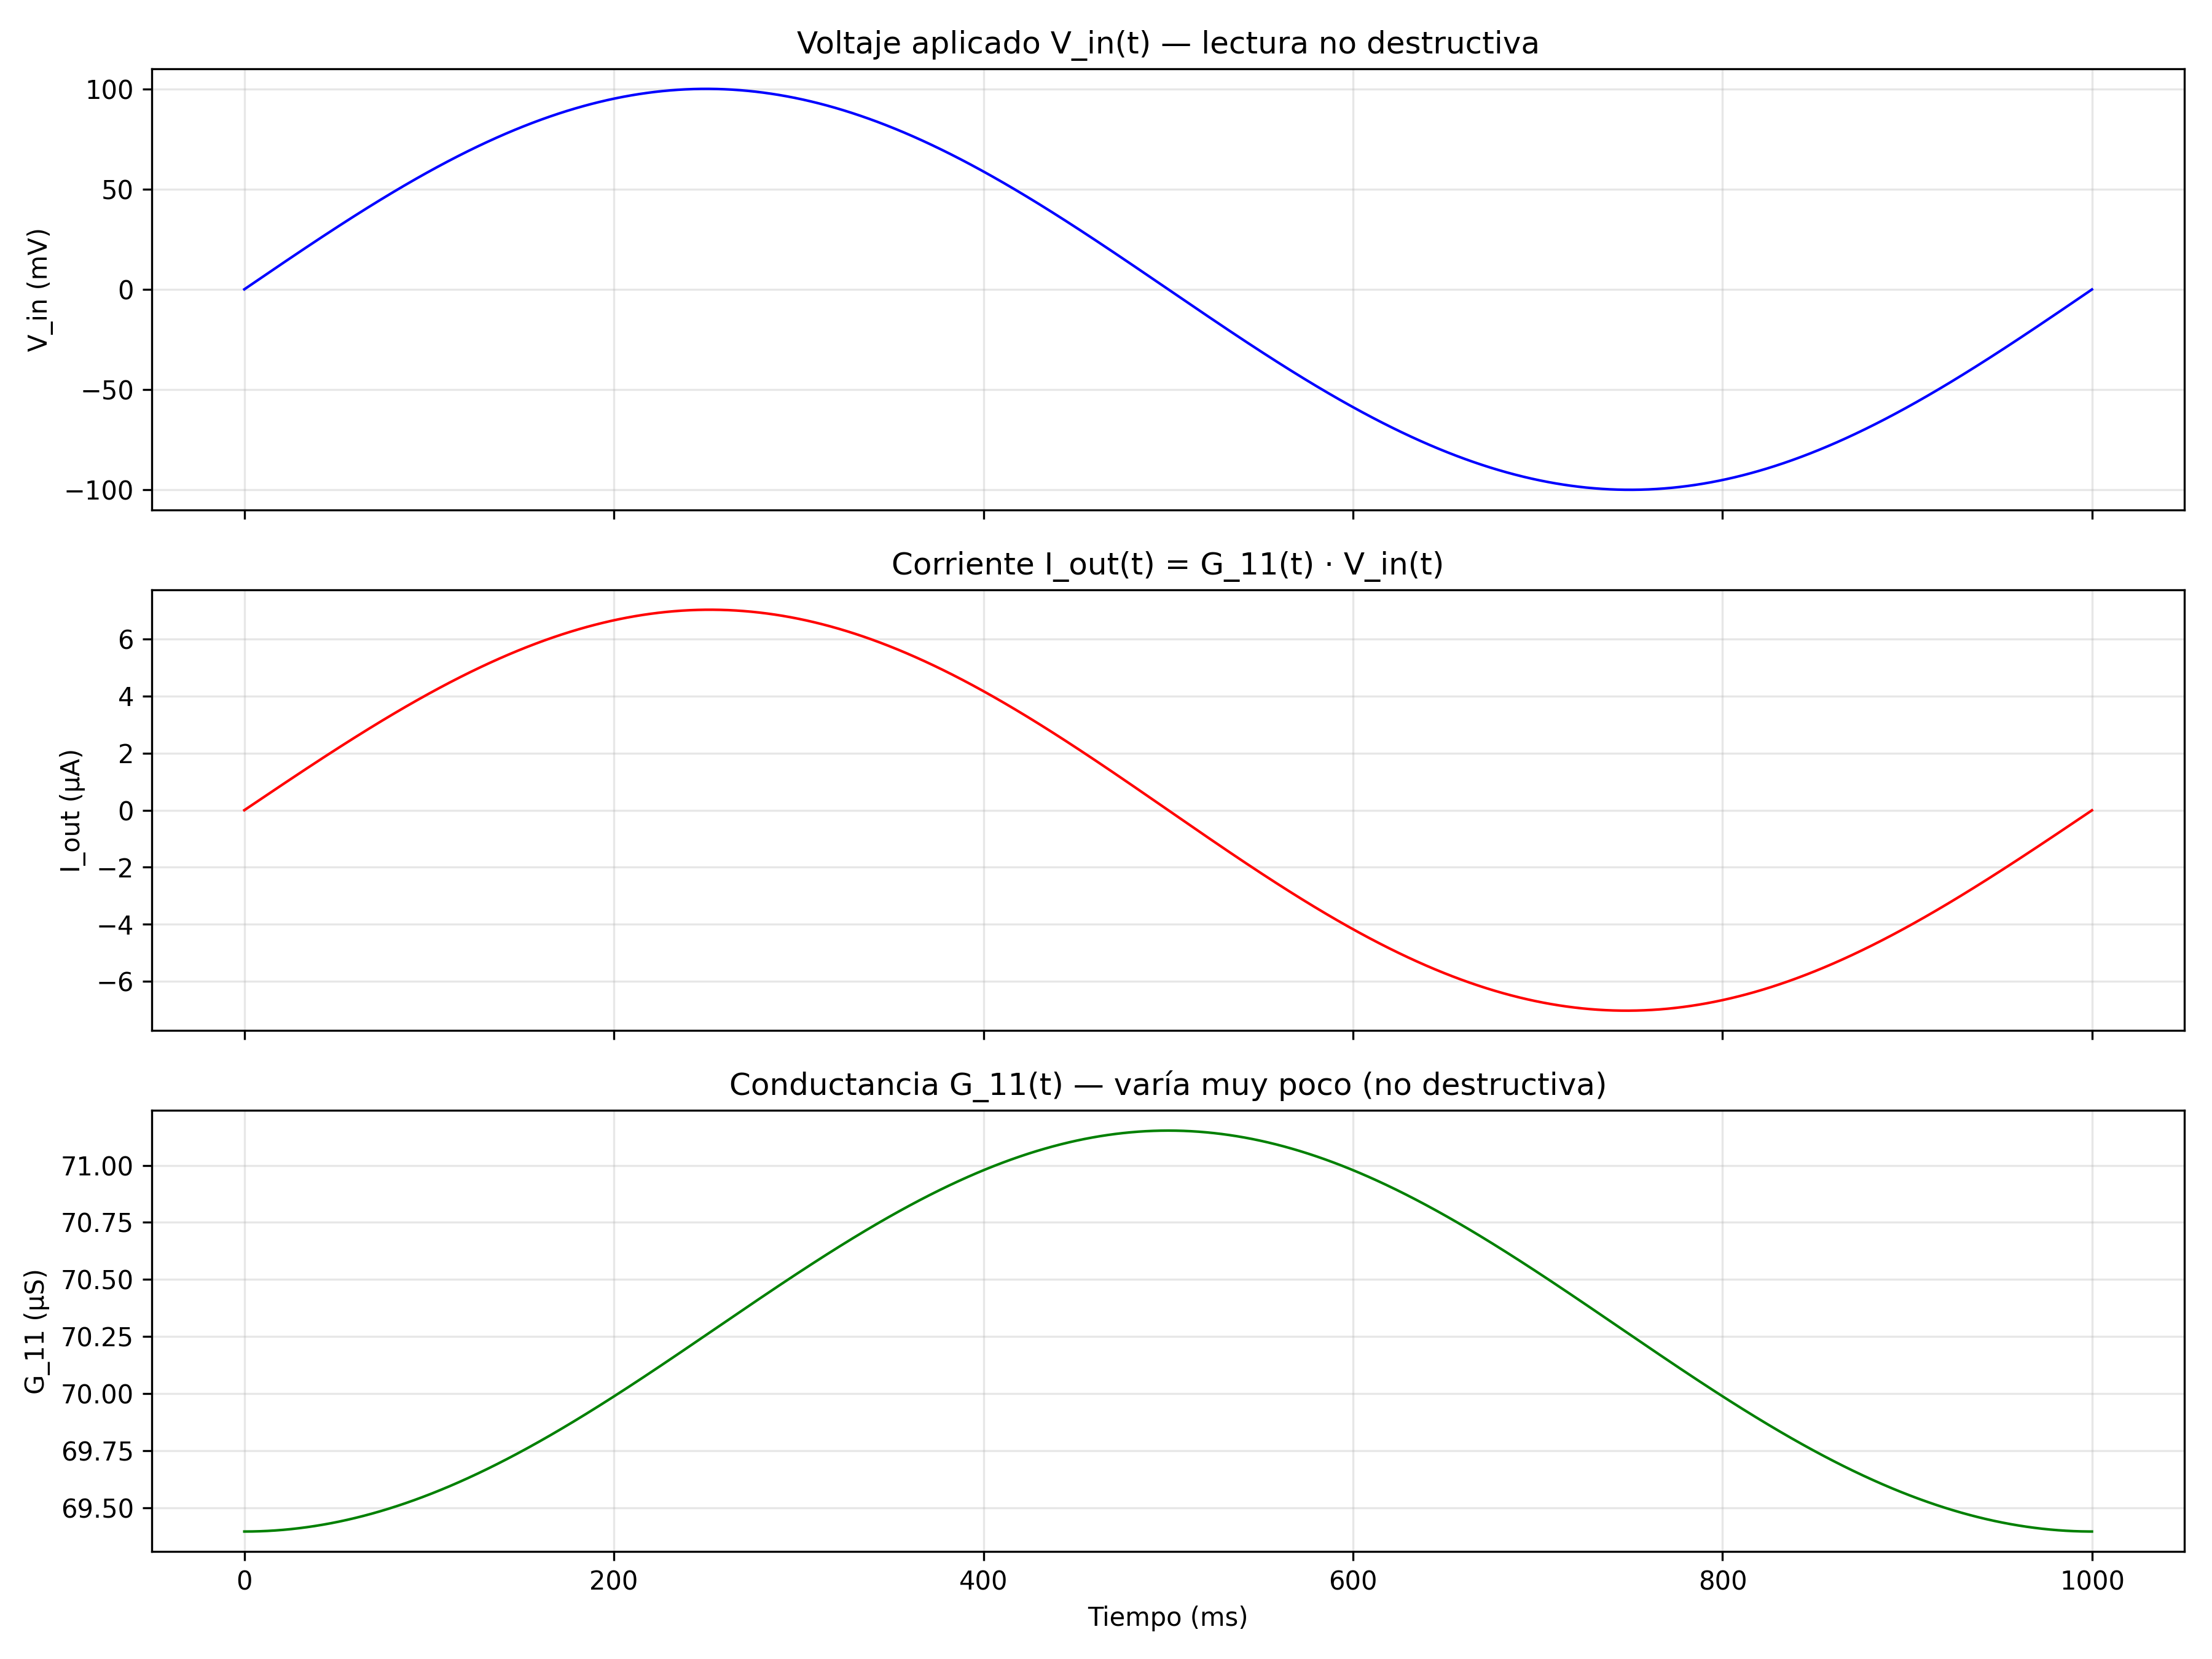
\includegraphics[width=\textwidth]{figuras/fig_21c_crossbar_din.png}
        \caption{Corrientes inferenciales recolectadas $I_j(t)$.}
    \end{subfigure}
    \vskip 0.3cm
    \begin{subfigure}[b]{0.84\textwidth}
        \centering
        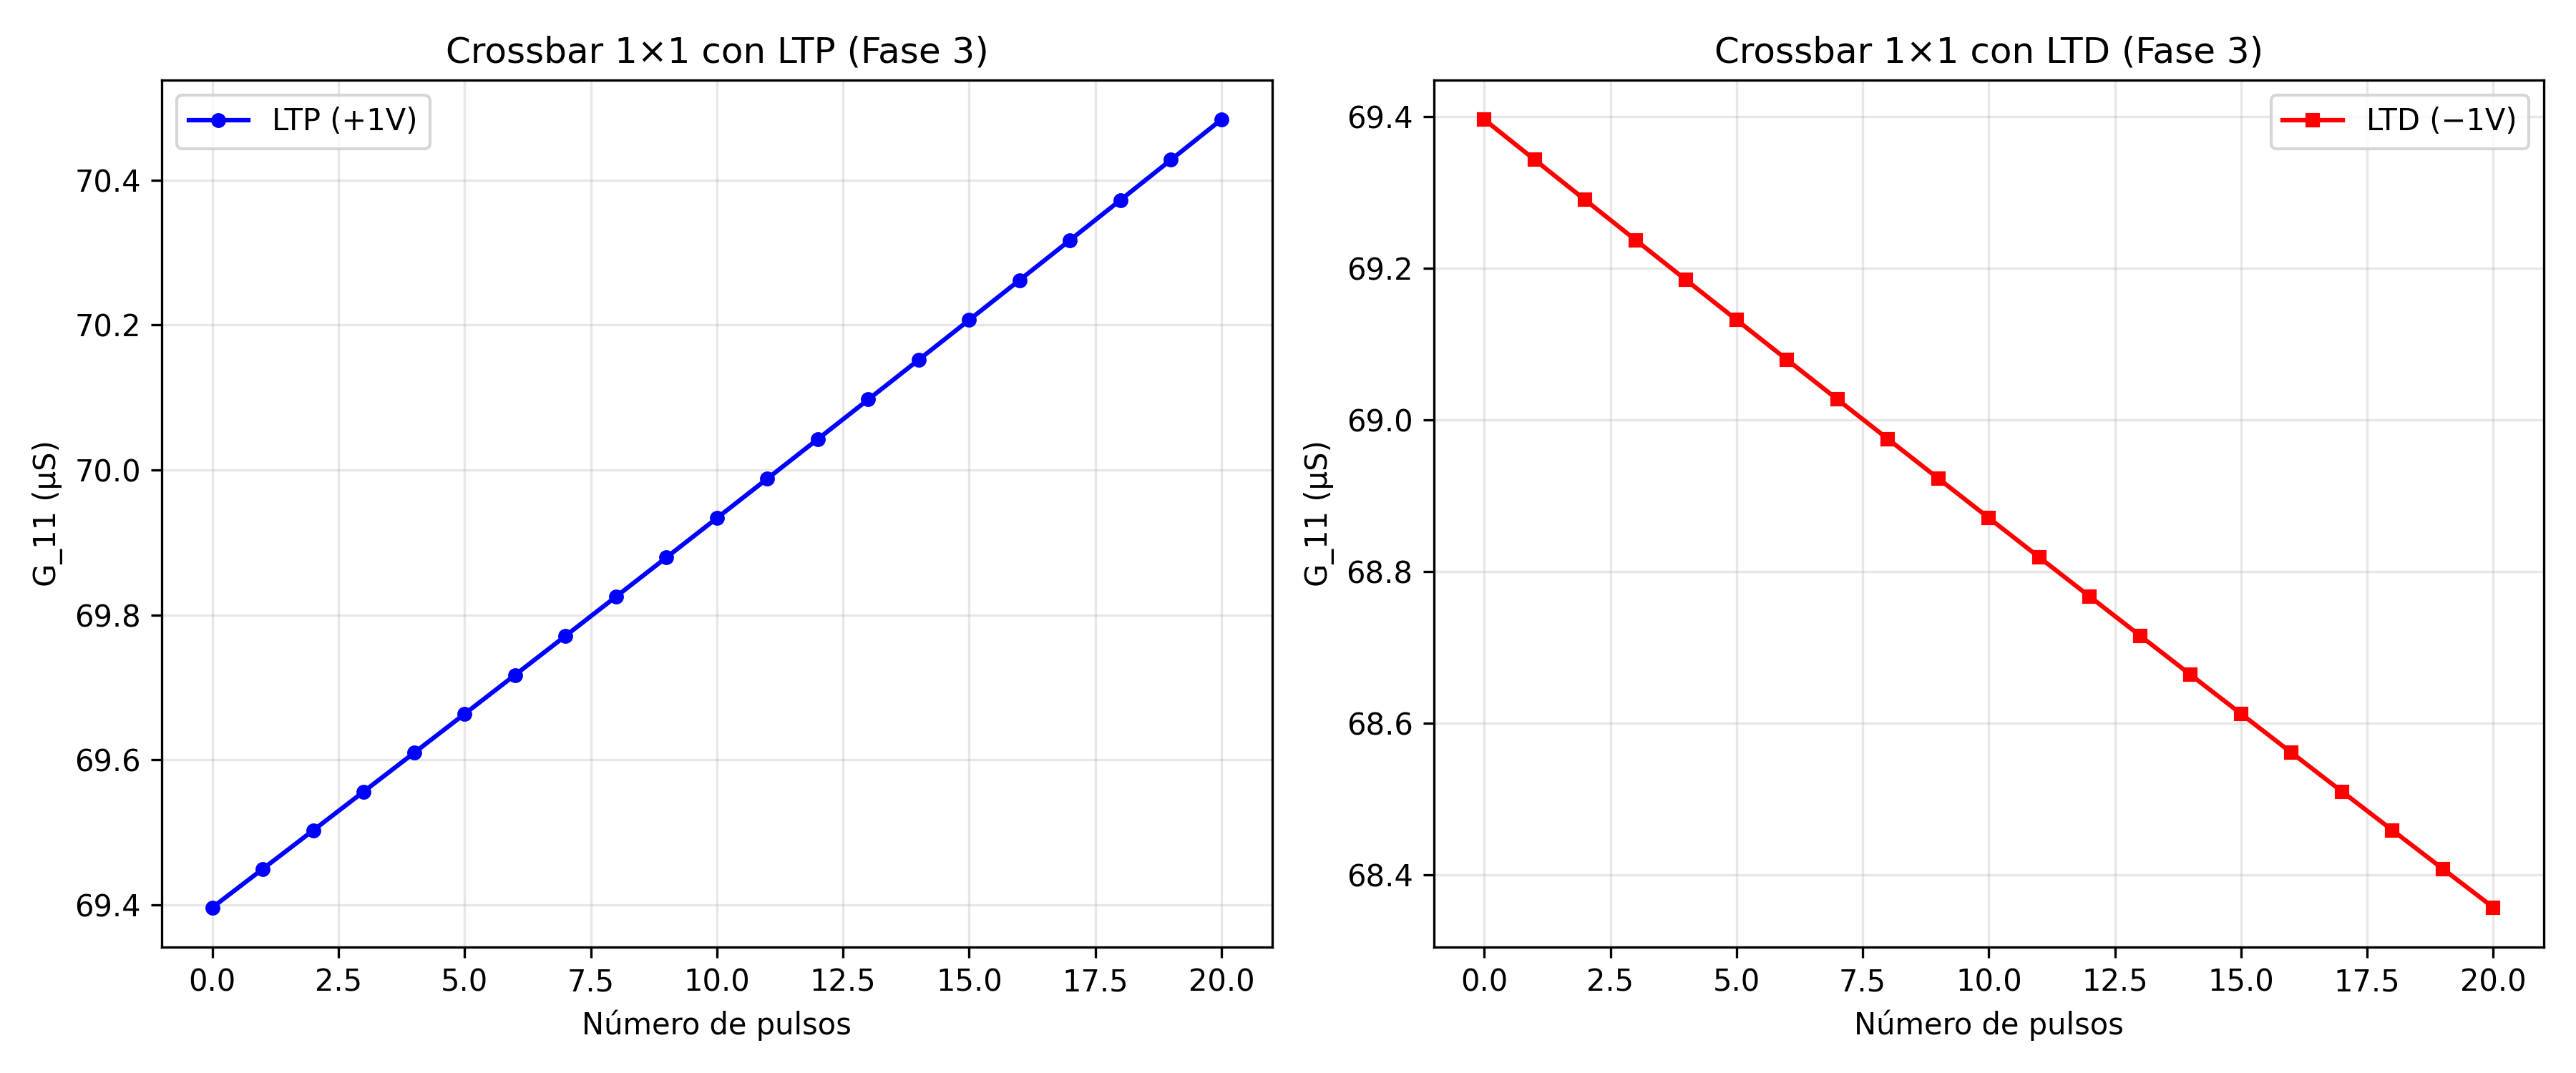
\includegraphics[width=\textwidth]{figuras/fig_21d_crossbar_stdp.png}
        \caption{Cinemática del oscilador memristivo de intersección.}
    \end{subfigure}
    \caption[]{(Continuación; paneles c y d).}
\end{figure}

\textbf{Propósito y Relevancia:} Los cuatro paneles ilustran señales y estados calculados por el modelo de simulación. No demuestran una implementación de hardware ni una ventaja temporal sobre un sistema digital.

\paragraph{Comparación cualitativa con Prezioso et al. (2015)}
La Figura~\ref{fig:prezioso_s3a} compara cualitativamente la forma de las curvas I--V generadas por el modelo local con las curvas representativas de dispositivos del panel S3a de Prezioso et al. (2015)~\cite{31}, correspondiente a la caracterización pre-forming de una porción de un crossbar $10 \times 8$. La comparación es de comportamiento y forma: el generador usa constantes locales y no carga ni digitaliza los puntos experimentales, por lo que no demuestra ajuste numérico ni concordancia punto por punto. Las Figuras~\ref{fig:prezioso_s3bc} muestran una matriz y un histograma sintéticos motivados por los paneles S3b--S3c; no reproducen las mediciones experimentales.

La curva de D-21 es paramétrica. D-22 usa una matriz sintética $4 \times 4$ de conductancias, generada con semilla fija a partir de una media y desviación estándar configuradas en el código. Ninguna de estas dos salidas representa mediciones de celdas reales ni valida ruido térmico o variabilidad medida.

\begin{figure}[H]
    \centering
    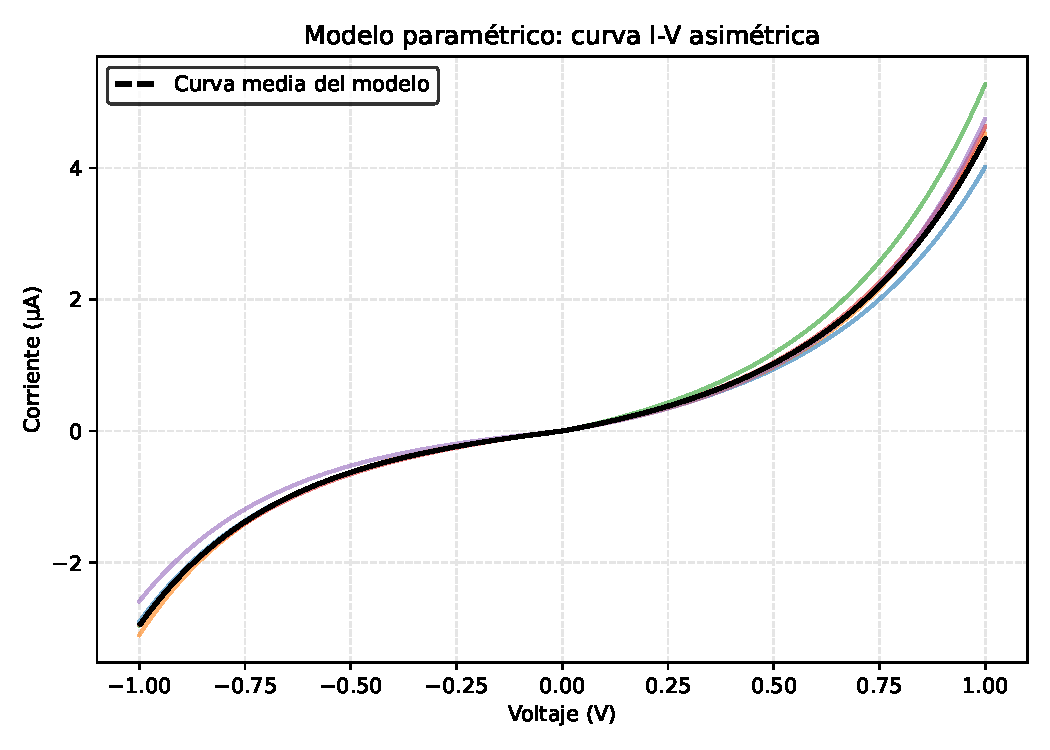
\includegraphics[width=0.85\textwidth]{figuras/23a_prezioso_s3a_modelo_ejemplo.pdf}
    \caption[Comparación cualitativa I-V con Prezioso S3a]{Comparación cualitativa de la forma I--V pre-forming con el panel S3a de Prezioso et al. (2015)~\cite{31}. Las curvas se generan con un modelo paramétrico local; no se cargan puntos digitalizados ni se afirma un ajuste cuantitativo.}
    \label{fig:prezioso_s3a}
\end{figure}

\textbf{Propósito y Relevancia:} Permite comparar visualmente el comportamiento asimétrico no lineal generado localmente con la forma de las curvas representativas del panel S3a. No acredita fidelidad de fabricación, ajuste numérico ni corrientes de fuga medidas.

\begin{figure}[H]
    \centering
    \begin{subfigure}[b]{0.48\textwidth}
        \centering
        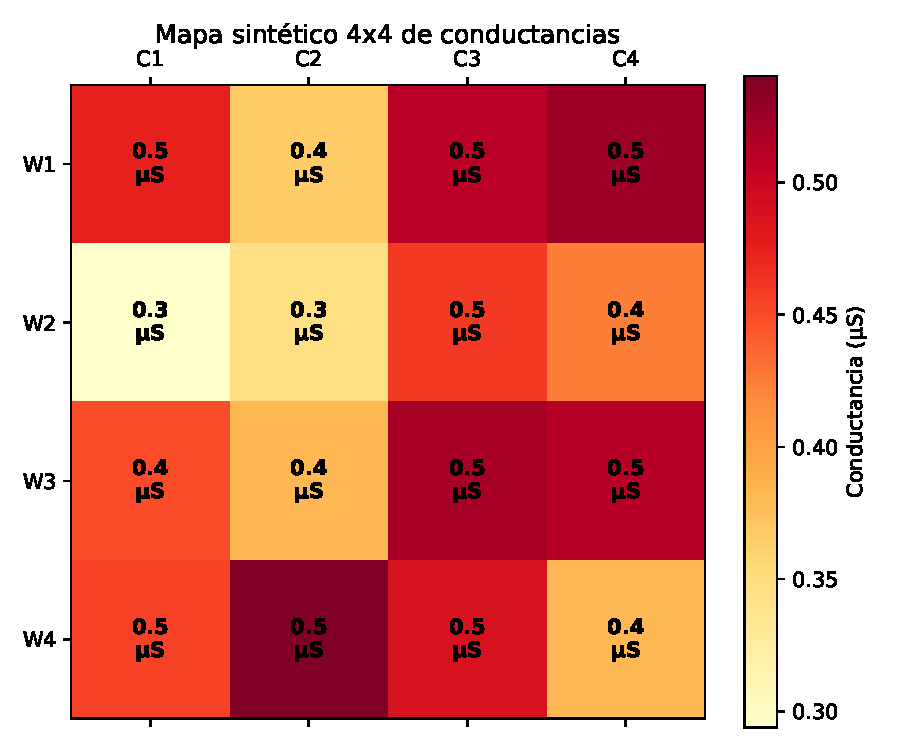
\includegraphics[width=\textwidth]{figuras/23b_prezioso_s3b_modelo_ejemplo.pdf}
        \caption{Matriz sintética de conductancias $4 \times 4$.}
    \end{subfigure}
    \hfill
    \begin{subfigure}[b]{0.48\textwidth}
        \centering
        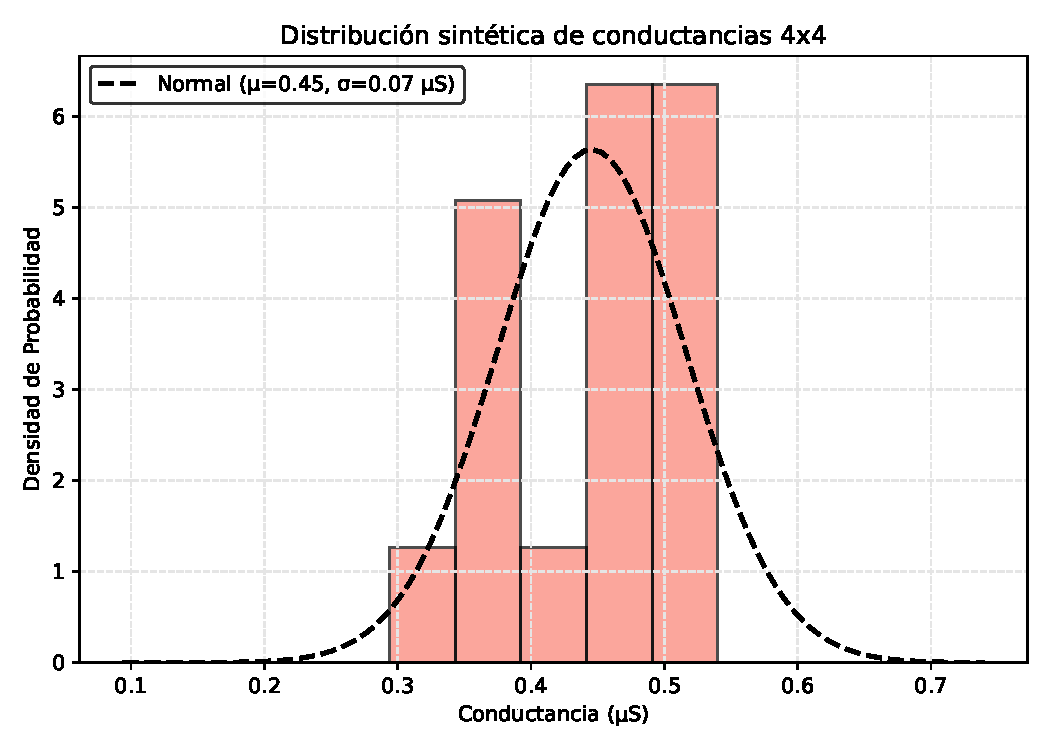
\includegraphics[width=\textwidth]{figuras/23c_prezioso_s3c_modelo_ejemplo.pdf}
        \caption{Histograma de la matriz sintética.}
    \end{subfigure}
    \caption[Ejemplos sintéticos de conductancia]{Ejemplos sintéticos de conductancias en una matriz $4 \times 4$ y su distribución. Los valores se generan en el simulador con semilla fija; no son mediciones ni una reproducción de las Figuras S3b--S3c de Prezioso et al. (2015)~\cite{31}.}
    \label{fig:prezioso_s3bc}
\end{figure}

\textbf{Propósito y Relevancia:} Ilustran la generación de una matriz virtual y un resumen estadístico de sus conductancias. No demuestran que la dispersión del simulador coincida con la variabilidad Device-to-Device del hardware reportado.

\begin{figure}[H]
    \centering
    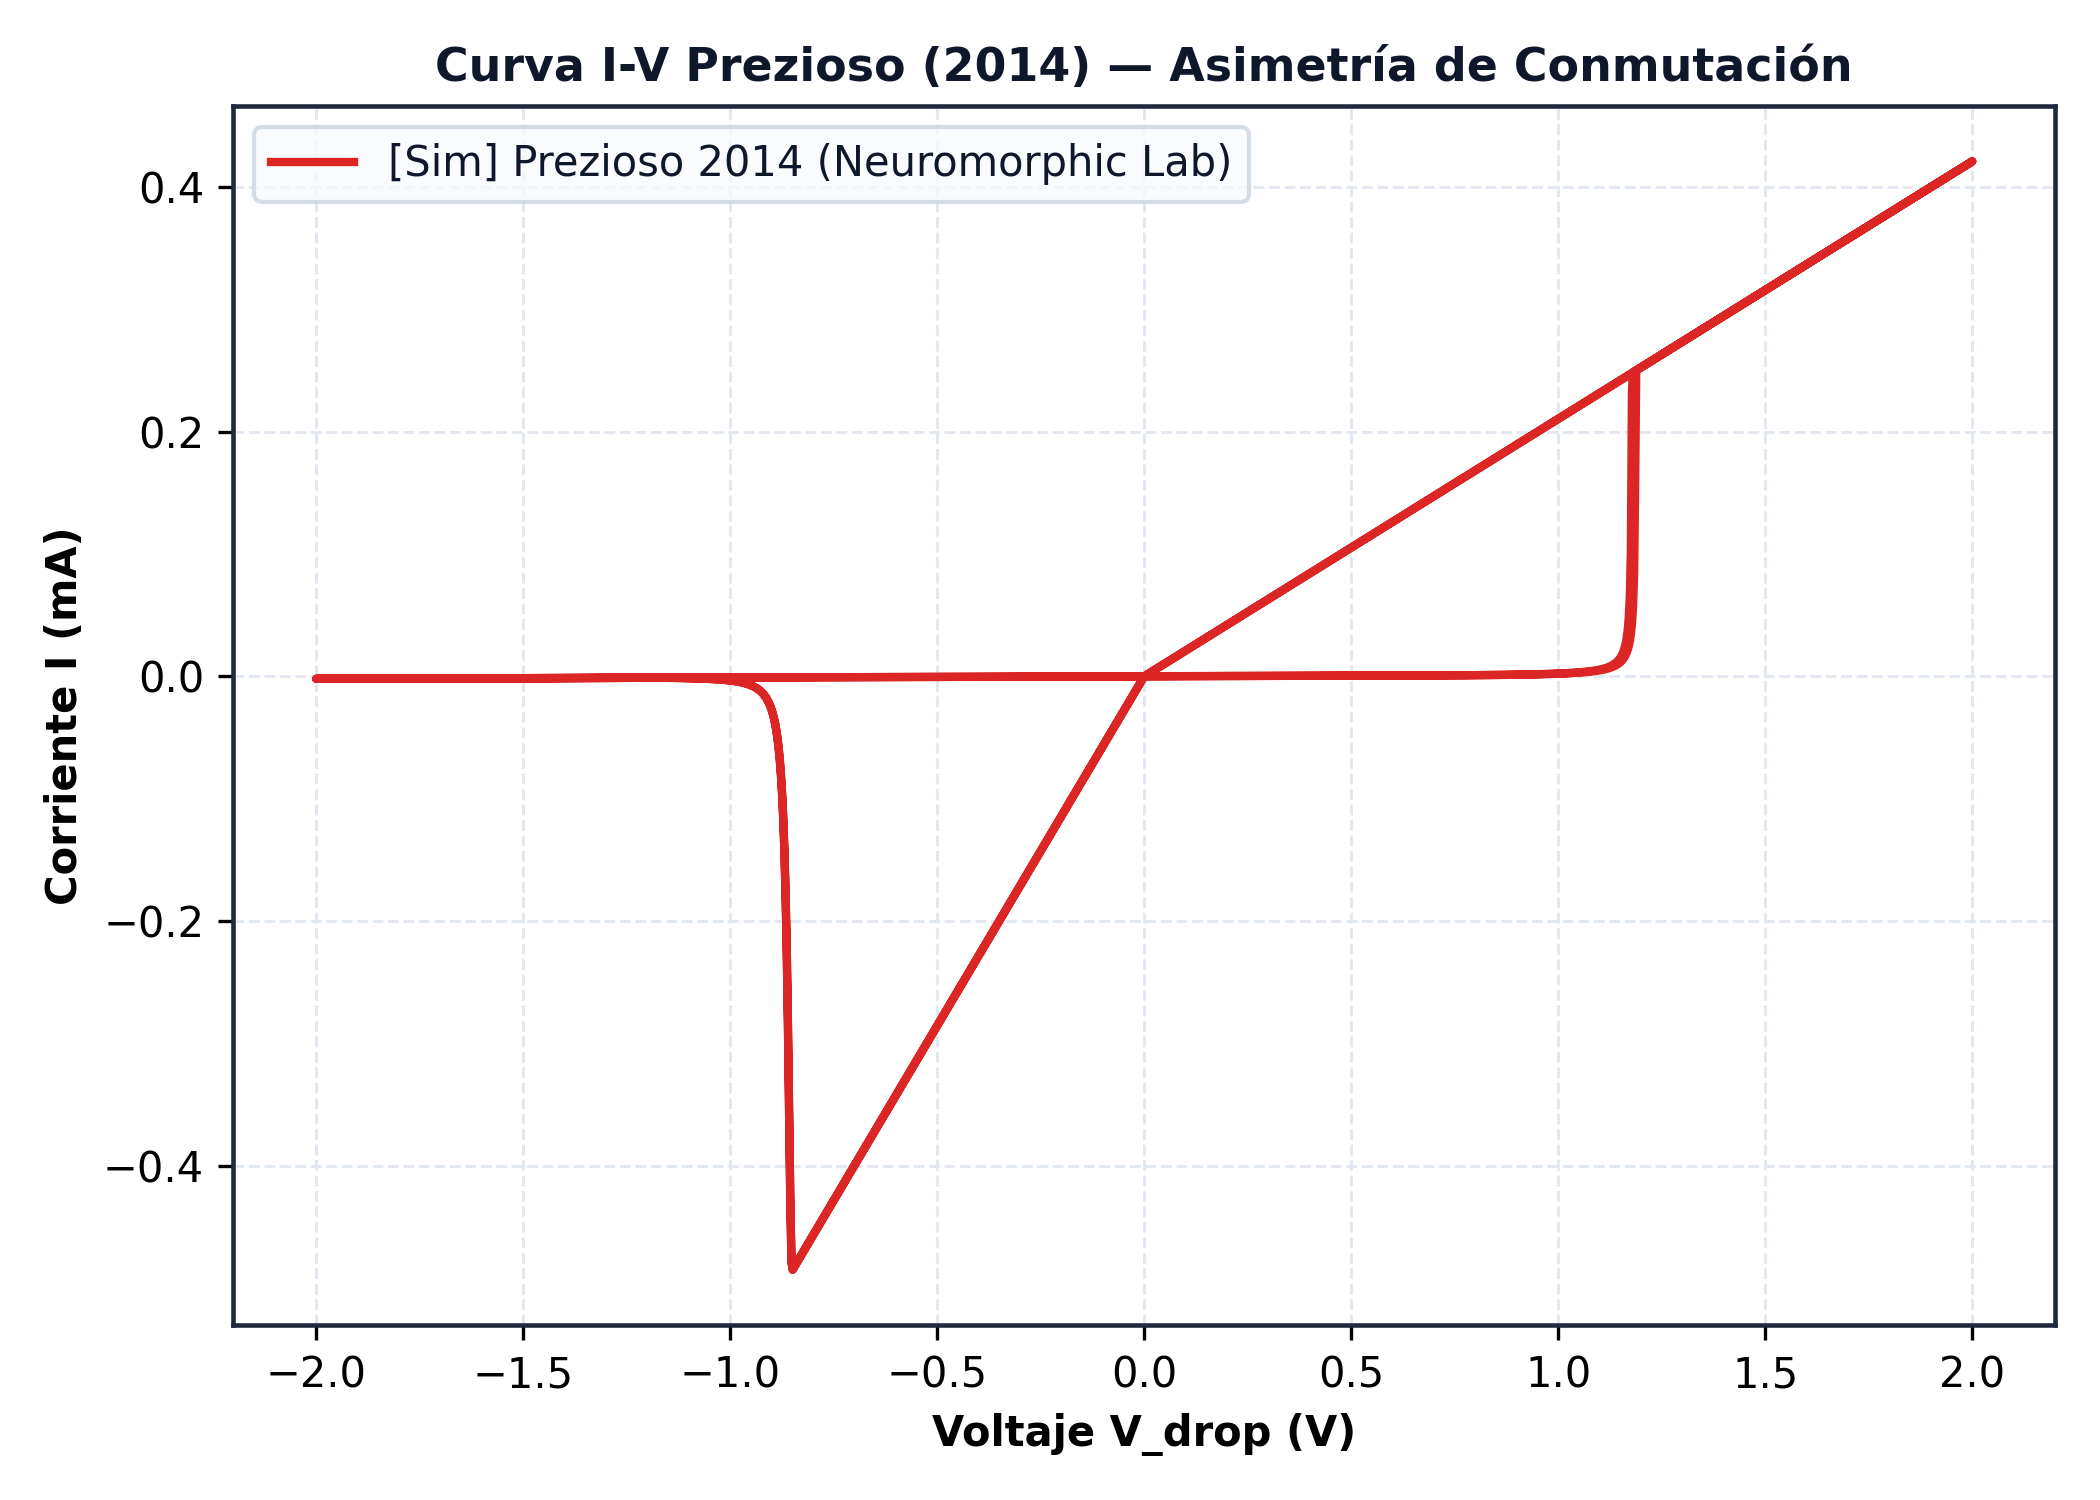
\includegraphics[width=0.7\textwidth]{figuras/fig_22_prezioso_v2.png}
    \caption{Respuesta I--V simulada con el modelo local inspirado en Prezioso et al. (2014)~\cite{3}. La curva se genera con parámetros configurados en el código; no incluye puntos experimentales ni constituye una validación cuantitativa del artículo.}
    \label{fig:22_prezioso_v2}
\end{figure}

\textbf{Propósito y Relevancia:} La figura muestra la respuesta I--V de una simulación local de un dispositivo bajo un barrido de voltaje. No muestra una matriz Crossbar ni prueba integración de sistema, escalamiento, operación SET/RESET en hardware o correspondencia cuantitativa con mediciones del artículo.


% =====================================================================
\subsubsection{Aplicación del crossbar al agente NeuroBot $24 \times 12$}
\label{sec:etapa4_2}

En esta sección se describe una arquitectura de aprendizaje por refuerzo (\textit{Reinforcement Learning}, RL) simulada: una red virtual de $24 \times 12$ acoplada al entorno CartPole. Los resultados son de simulación y no representan una validación experimental en hardware robótico o memristivo.

\paragraph{Arquitectura del Sistema ($24 \times 12$)}
El cerebro neuromórfico del agente consiste en un crossbar memristivo de $N=24$ filas de entrada y $M=12$ columnas de salida.

\subparagraph{Codificador de Estados (Encoder Top-K)}
El vector de observación continuo $\mathbf{s} = [x, \dot{x}, \theta, \dot{\theta}] \in \mathbb{R}^4$ se proyecta mediante una batería de receptores gaussianos distribuidos a lo largo del dominio de cada variable. Se aplica un mecanismo Top-K ($K=10$) que selecciona las 10 filas de mayor activación, generando un patrón binario disperso de voltajes de lectura $V_{\text{rows}} \in \{0, V_{\text{read}}\}$.

\subparagraph{Crossbar Memristivo y Solución Nodal (MNA)}
La corriente integrada por columna $\mathbf{I}_{\text{col}} \in \mathbb{R}^{12}$ se calcula resolviendo la matriz MNA con resistencia de línea $R_{\text{wire}} = 10^{-3}\,\Omega$ y resistencia de sensado $R_{\text{sense}} = 100\,\Omega$:
\begin{equation}
    \mathbf{I}_{\text{col}} = \text{MNA}(\mathbf{G}, V_{\text{rows}}, R_{\text{wire}}, R_{\text{sense}})
\end{equation}
donde $G_{ij} = \frac{1}{R_{\text{on}} + X_{ij}(R_{\text{off}} - R_{\text{on}})}$ representa la conductancia de la celda en el estado interno $X_{ij} \in [0, 1]$.

\subparagraph{Decodificador y Acción (Softmax e Inercia de Motor)}
Las 12 columnas se agrupan en pares de conductancias asociadas a 6 niveles discretos de fuerza activa para giro hacia la izquierda ($1 - 30\,\text{N}$) y 6 para la derecha ($1 - 30\,\text{N}$). La probabilidad de selección de acción $\pi_j$ sigue una distribución Softmax parametrizada por la temperatura ambiental $T$:
\begin{equation}
    \pi_j = \frac{\exp(I_j / T)}{\sum_{k=1}^M \exp(I_k / T)}
\end{equation}
Se aplica una tasa de cambio (slew rate) de $50/50$ en la dinámica del actuador para simular la inercia del motor robótico real.

\paragraph{REINFORCE con baseline}
El aprendizaje del agente no es STDP: es REINFORCE con baseline y ocurre al final de cada episodio:
\begin{equation}
    \Delta X_{ij} = -\eta \cdot E_{ij} \cdot (R_{\text{ep}} - b)
\end{equation}
donde $E_{ij}$ es la elegibilidad acumulada por paso a partir de $\mathrm{pre}_i(t)(\mathbf{1}_{j=a(t)}-\pi_j(t))$, con decaimiento $\gamma$ entre pasos. No se usa una ventana de STDP entre disparos pre y postsinápticos ni una traza de memristores volátiles; $E$ se mantiene como acumulador matemático del agente.

Con la convención $X=1-x$, una ventaja positiva produce
$\Delta X<0$ en la columna elegida cuando su elegibilidad es positiva;
esto reduce su resistencia y aumenta su conductancia. La prueba
unitaria del agente comprueba este signo en un caso controlado, sin
demostrar convergencia general ni equivalencia con STDP.

La actualización $\Delta X$ utiliza recorte por norma de gradiente
($\max|\Delta X| \le 0.05$) y se congela si
$R_{\text{ep}} \ge 430$. Este umbral es un criterio operativo del
protocolo evaluado y no demuestra que la política alcanzada sea óptima.

\paragraph{Resultados de simulación y discusión en control robótico}

Los valores de recompensa y ablación de esta sección proceden de
registros de simulación previamente reportados. No se reejecutaron las
cinco semillas ni las ablaciones durante esta revisión; por tanto, se
presentan como resultados reportados, no como cifras reproducidas aquí
ni como resultados experimentales de hardware.

\subparagraph{Convergencia y Reproducibilidad Multi-Semilla}
Se ejecutaron cinco semillas (0--4), con 300 episodios cada una, $V_{\mathrm{read}}=0.05$ V, D2D ($\sigma=0.08$), C2C ($\sigma=0.05$, $\theta=1\,\mathrm{s}^{-1}$, $dt=0.02\,\mathrm{s}$) y congelamiento de la actualización de pesos para $R_{\mathrm{ep}}\geq430$. Las recompensas medias de los últimos 200 episodios fueron 369.66, 421.44, 474.31, 462.79 y 448.36, respectivamente; la media entre semillas fue 435.31 y su desviación estándar 37.28. Cuatro corridas alcanzaron al menos una recompensa episódica de 480; la semilla 3 tuvo máximo 479.14. Los registros se guardan como \texttt{run\_24x12\_A\_d2d\_c2c\_seed0.json}--\texttt{seed4.json}; la figura y discusión se presentan en la Sección~3.4.1.

La media de la semilla 0 debe interpretarse considerando su trayectoria:
las recompensas medias por bloques de 50 episodios fueron 13.90,
58.55, 99.39, 470.69, 461.27 y 447.29. Su primera media móvil de
20 episodios que alcanzó 430 apareció en el episodio 157. Así, el
promedio de los episodios 101--300 (369.66) refleja en buena medida el
tiempo que tardó esta corrida en alcanzar recompensas altas y no basta
para concluir que la semilla sea intrínsecamente peor. Este cruce es
un indicador operativo de adquisición de desempeño, no una
demostración formal de convergencia; el análisis detallado se presenta
en la Sección~\ref{sec:res_cartpole}.

\subparagraph{Estudio de Ablaciones}
Para validar la contribución de cada bloque del agente, se evaluaron cuatro configuraciones (Figura~\ref{fig:ablaciones_robot}):
\begin{itemize}
    \item \textbf{A (Control Base):} Sistema completo con decaimiento térmico y traza acumulativa ($\bar{R} \approx 491.9$ en semillas exitosas, $60\%$ de tasa de convergencia en 5 semillas aleatorias).
    \item \textbf{B (Sin Adaptación Térmica, $T=0.10$ Fijo):} Colapso por congelamiento estocástico ($\bar{R} = -39.0$). Demuestra que sin alta exploración inicial, el agente congela la búsqueda de políticas.
    \item \textbf{C (Sin Traza de Elegibilidad, $\varepsilon=0$):} Colapso total ($\bar{R} = -33.3$, $\Delta X=0$), evidenciando que la elegibilidad acumulada es necesaria en la configuración REINFORCE evaluada.
    \item \textbf{D (Hebbiano Sin Modulación $R_{\text{ep}}-b$):} Divergencia y colapso ($\bar{R} = -39.0$) por falta del escalar de refuerzo global.
\end{itemize}

\begin{figure}[H]
    \centering
    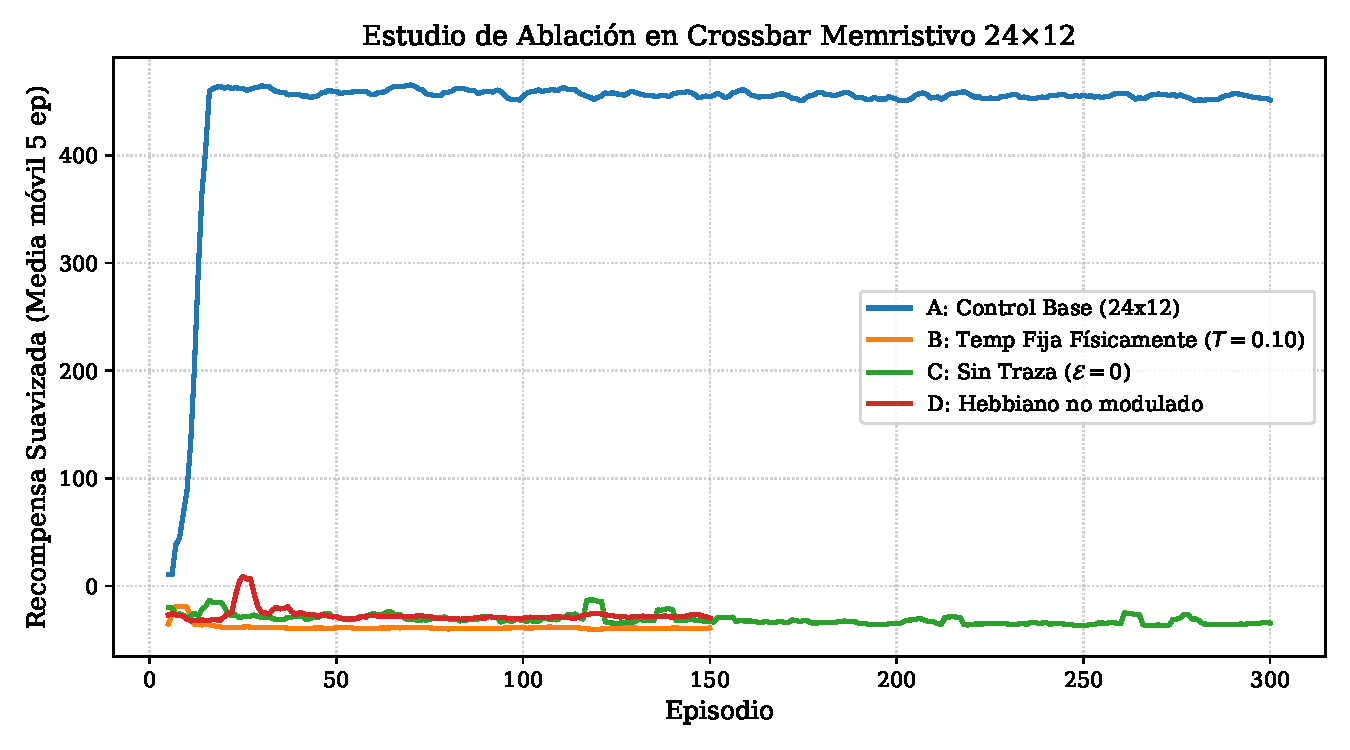
\includegraphics[width=0.85\textwidth]{figuras/comparativa_ablaciones_24x12.pdf}
    \caption{Estudio de ablación comparativo (A, B, C, D) en el crossbar $24 \times 12$.}
    \label{fig:ablaciones_robot}
\end{figure}

\subparagraph{Heatmap de la Matriz Memristiva Consolidada ($X$)}
La Figura~\ref{fig:heatmap_robot} muestra la distribución final del estado memristivo $X \in [0, 1]$. Se observa una estructura bimodal no saturada ($\mu = 0.165, \sigma = 0.118$) con bandas claras de activación sináptica diferenciadas por la velocidad y el ángulo del poste.

\begin{figure}[H]
    \centering
    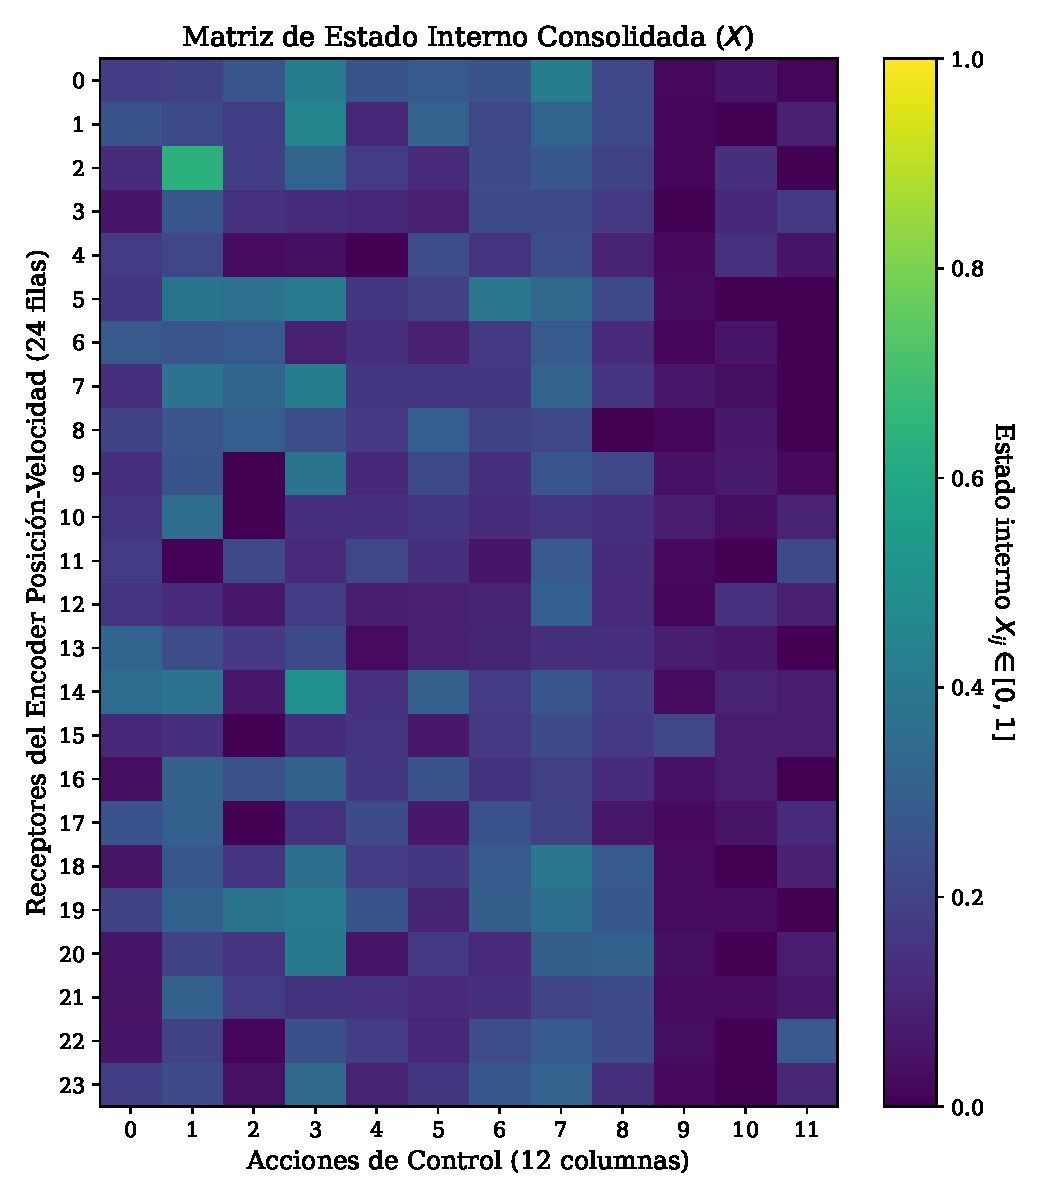
\includegraphics[width=0.65\textwidth]{figuras/heatmap_matriz_X_24x12.pdf}
    \caption{Heatmap de la variable de estado interno $X$ tras el entrenamiento del agente; la conductancia $G$ se deriva de $X$ y no se muestra en esta figura.}
    \label{fig:heatmap_robot}
\end{figure}


% =====================================================================
\subsubsection{Validación del Modelo Físico del Crossbar (Suite de 10 Experimentos)}
\label{sec:suite_10_exp}

La suite consta de 10 experimentos de simulación autónomos del modelo
crossbar. Las cifras que siguen son las consignadas en sus informes y
figuras existentes; no se reejecutaron ni se verificaron de nuevo sus
registros de entrada en esta revisión. Por ello describen resultados
reportados del modelo, no una certificación de fidelidad respecto a
hardware real. Las condiciones de excitación y las impedancias de
sensado ($R_{\text{sense}} = 100\,\Omega$) se atribuyen a la
configuración declarada para el agente.

\paragraph{Exp.~1 --- Error de lectura del crossbar vs.\ tamaño}

La Figura~\ref{fig:exp01} cuantifica el error relativo de lectura del arreglo
al escalar de $N=4$ a $N=32$ filas con $M=12$ columnas fijas. Se define el
error relativo como
$\varepsilon = \|I_{\text{col}} - I_{\text{ideal}}\| / \|I_{\text{ideal}}\|$,
donde $I_{\text{col}}$ es la solución nodal del arreglo (MNA con
$R_{\text{wire}}$ y $R_{\text{sense}}$) e $I_{\text{ideal}} = \mathbf{G}^T \mathbf{V}$
es la proyección lineal ideal.

Para $N=4$ el error es $\varepsilon \approx 6.5\%$ y escala monótonamente
hasta $\varepsilon \approx 41\%$ para $N=32$. Este crecimiento refleja la
contribución conjunta de la caída resistiva en las líneas ($R_{\text{wire}}$)
y el divisor formado por $R_{\text{sense}}$ con la conductancia agregada del
arreglo. El efecto de corrientes parásitas estrictas (\textit{sneak paths} en
el sentido clásico: fila única activa con filas flotantes) requiere una
configuración de excitación distinta y se considera una extensión natural
para trabajos futuros.

\begin{figure}[H]
  \centering
  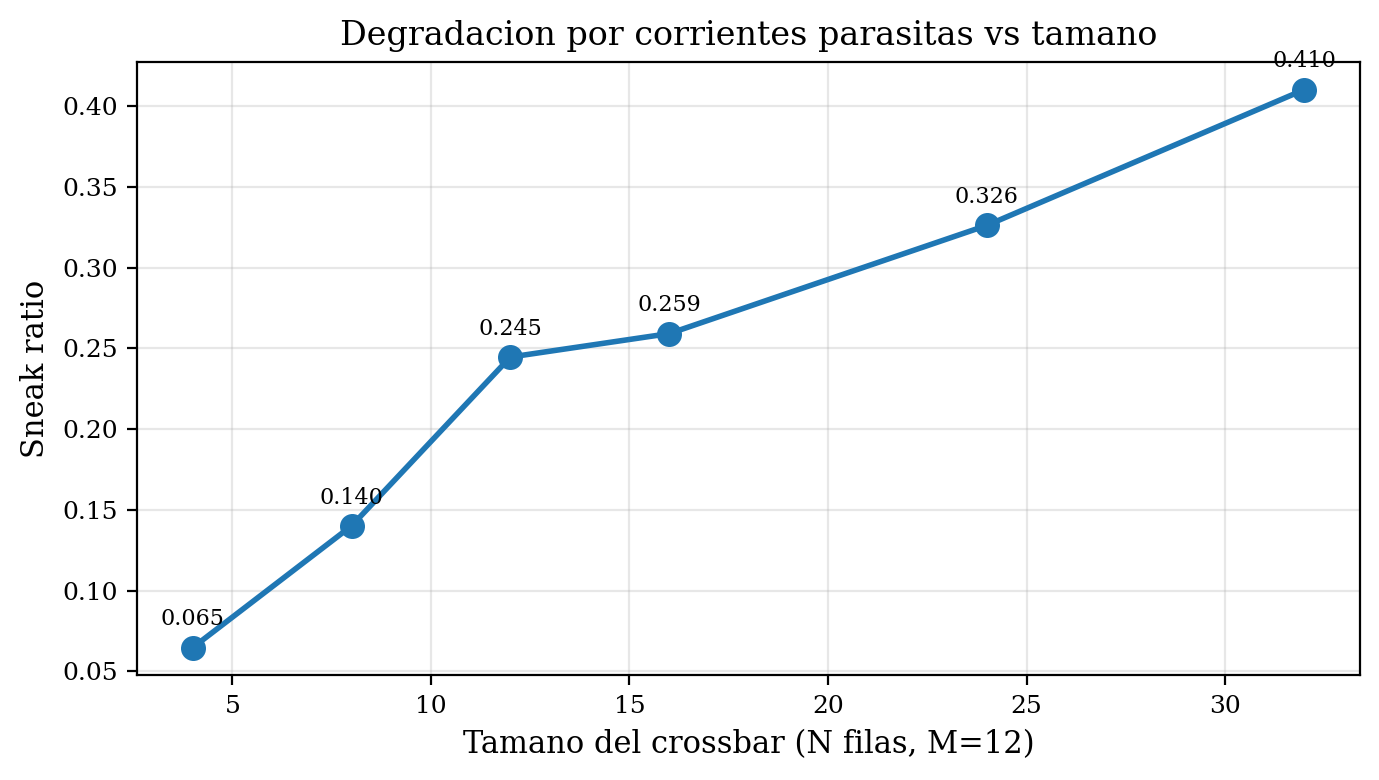
\includegraphics[width=0.65\textwidth]{experiments/figures/exp01_sneak_vs_N.png}
  \caption{Error relativo de lectura vs.\ tamaño del arreglo. Crecimiento
  monótono desde $N=4$ ($6.5\%$) hasta $N=32$ ($41\%$).}
  \label{fig:exp01}
\end{figure}

\paragraph{Exp.~2 --- MNA real vs.\ modelo ideal}
La Figura~\ref{fig:exp02} compara corrientes MNA e ideales para cuatro tamaños. En el caso $N=24$, el error medio por componente alcanza $29.08\%$, reflejando la contribución acumulada de $R_{\text{wire}}$ y $R_{\text{sense}}$ sobre las corrientes de columna.
\begin{figure}[H]
  \centering
  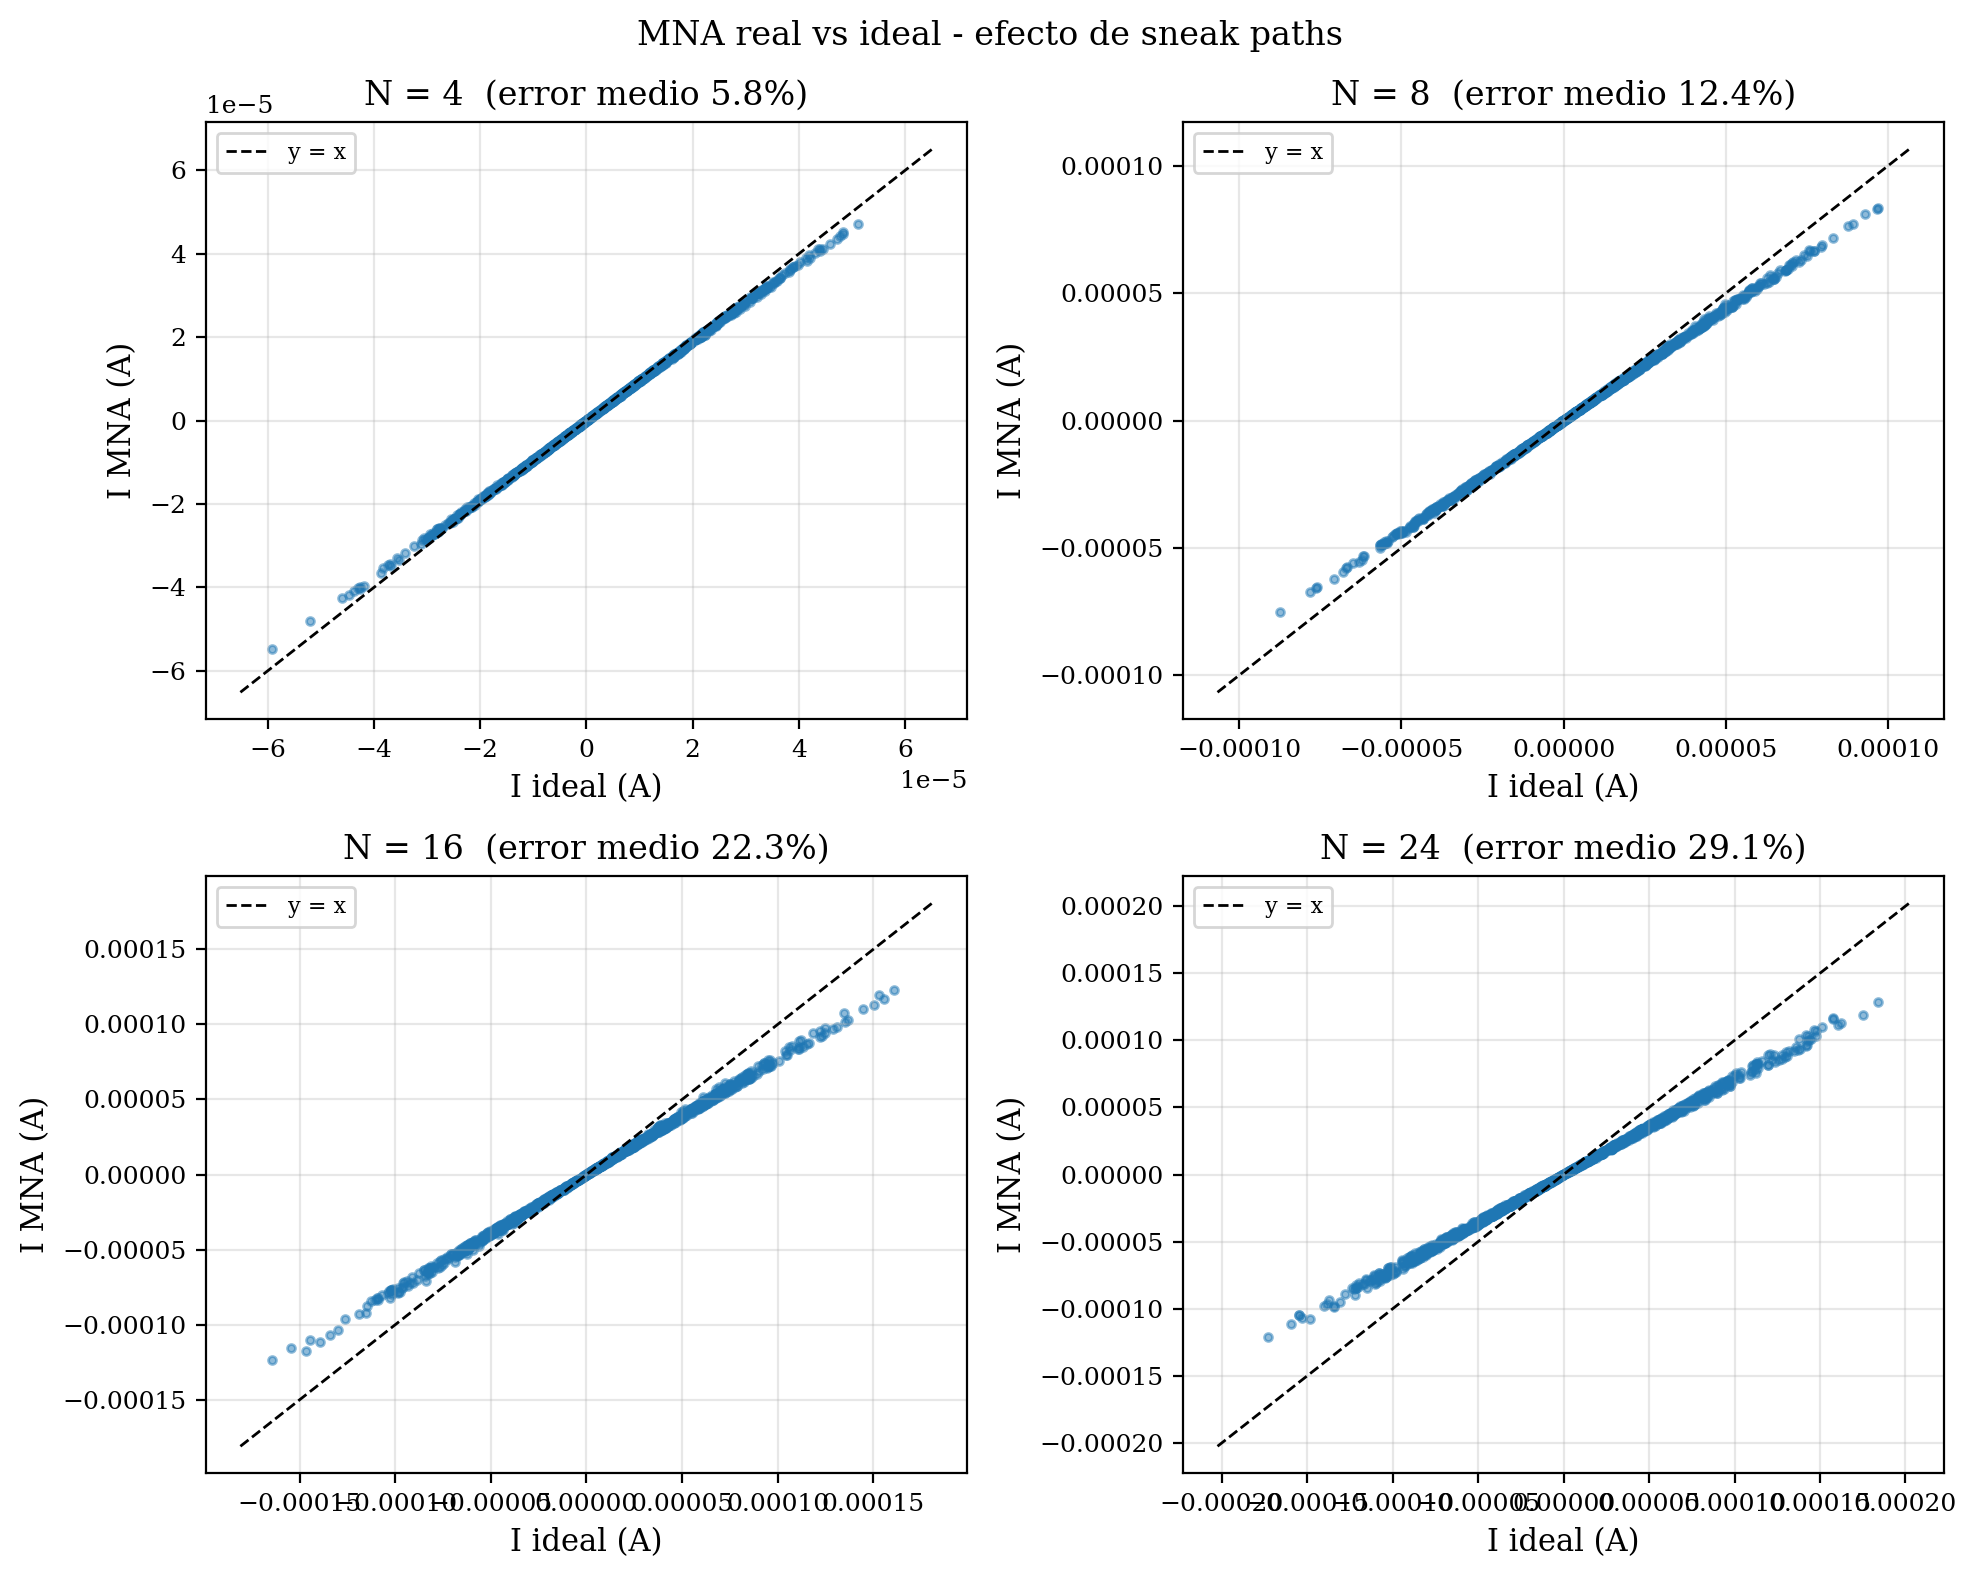
\includegraphics[width=0.90\textwidth]{experiments/figures/exp02_mna_vs_ideal.png}
  \caption{Diagrama de dispersión MNA vs.\ Ideal. El error crece de forma no lineal con $N$.}
  \label{fig:exp02}
\end{figure}

\paragraph{Exp.~3 --- Caída de tensión en línea ($R_{\text{wire}}$)}
La Figura~\ref{fig:exp03} ilustra cómo $R_{\text{wire}}$ distorsiona el perfil de corriente. El efecto sobre el perfil es doble: atenúa la corriente media ($-13\%$ entre $R_{\text{wire}} = 1\,\text{m}\Omega$ y $R_{\text{wire}} = 10\,\Omega$) y mantiene prácticamente invariante la no-uniformidad relativa entre columnas ($\sim 27\%$), dominada por la dispersión dispositivo-a-dispositivo de $\mathbf{G}$.
\begin{figure}[H]
  \centering
  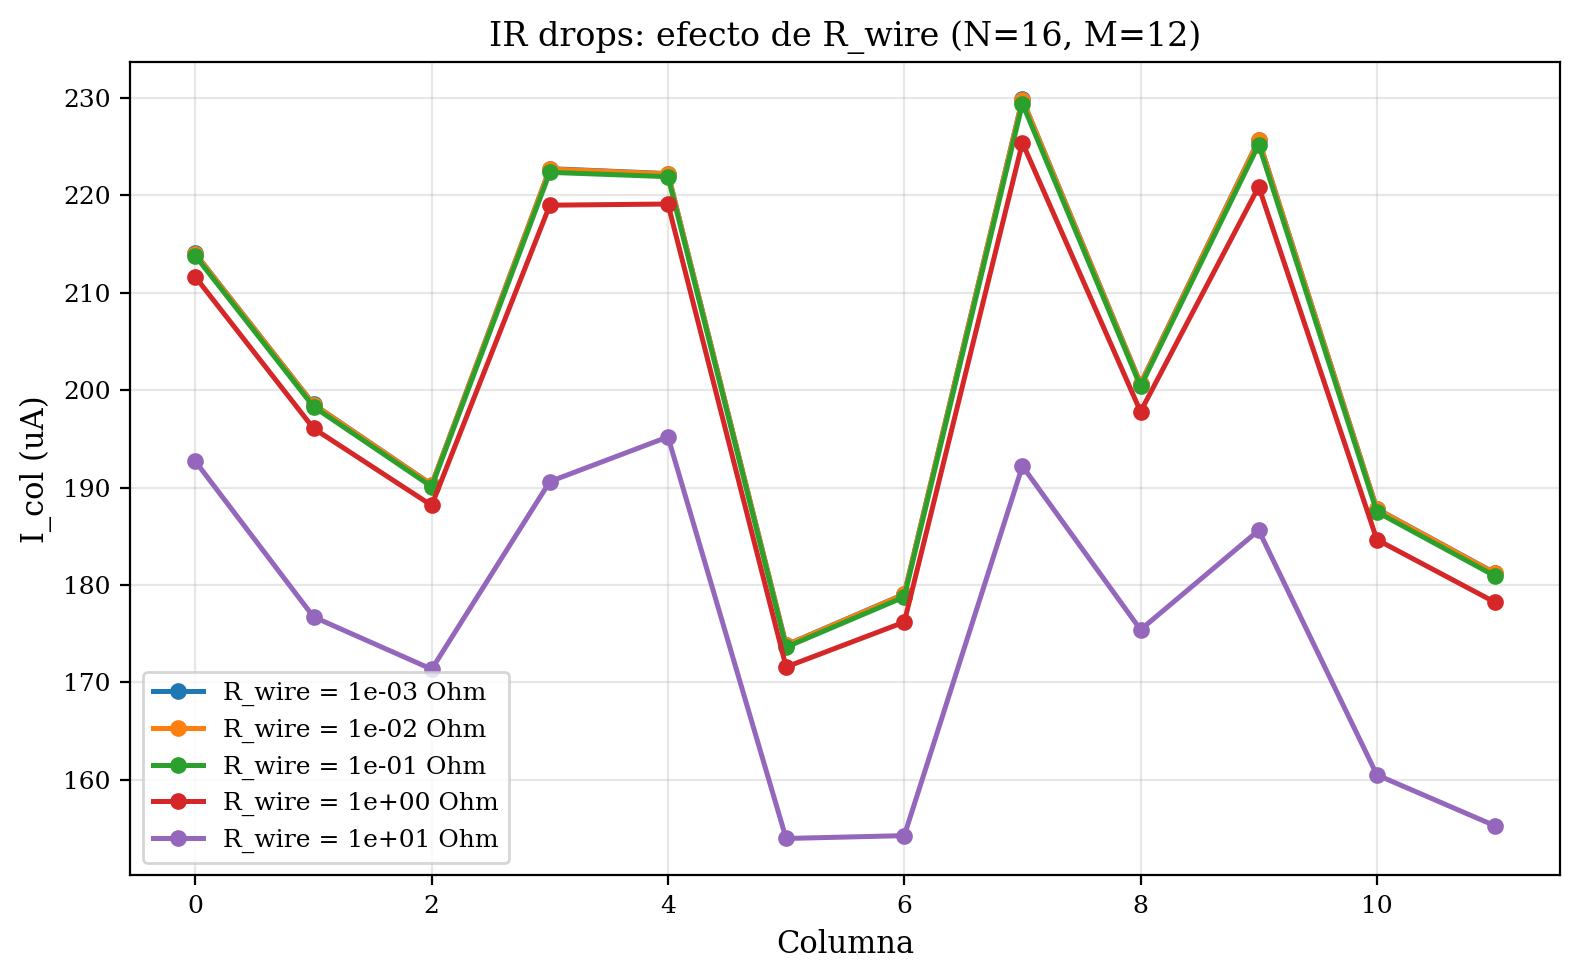
\includegraphics[width=0.72\textwidth]{experiments/figures/exp03_rwire_effect.png}
  \caption{Perfil de $I_{\text{col}}$ para distintos $R_{\text{wire}}$. La
atenuación de la corriente media aumenta con la resistencia de línea, mientras
que la dispersión entre columnas se mantiene dominada por la variabilidad de
$\mathbf{G}$.}
  \label{fig:exp03}
\end{figure}

\paragraph{Exp.~4 --- Precisión en VMM}
La Figura~\ref{fig:exp04} muestra la distribución del error relativo en VMM para 1000 vectores aleatorios. El error medio crece de $5.82\%$ ($N=4$) a $29.05\%$ ($N=24$).
\begin{figure}[H]
  \centering
  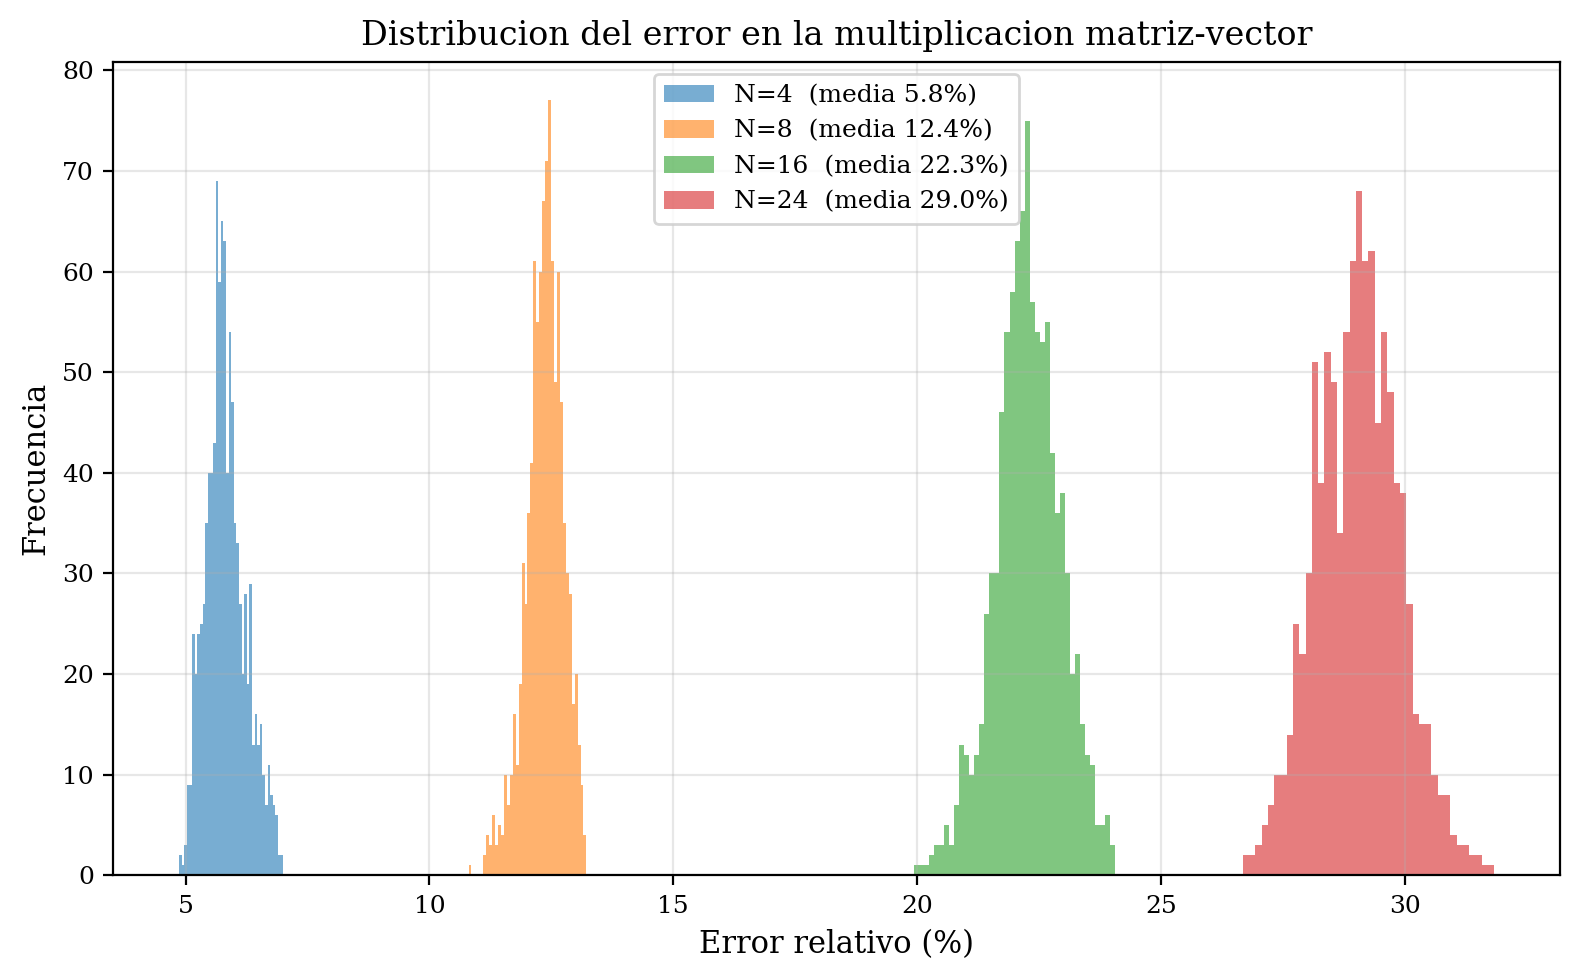
\includegraphics[width=0.70\textwidth]{experiments/figures/exp04_vmm_precision.png}
  \caption{Histograma del error relativo en VMM por tamaño de crossbar.}
  \label{fig:exp04}
\end{figure}

\paragraph{Exp.~5 --- Half-select disturb simulado: V/2 vs.\ V/3}
La Figura~\ref{fig:exp05} compara la perturbación calculada por el modelo para celdas \textit{half-selected}. Los valores reportados son 50.0\% para V/2 y 33.3\% para V/3; son razones de excitación del protocolo simulado, no medidas de disturb en celdas fabricadas.
\begin{figure}[H]
  \centering
  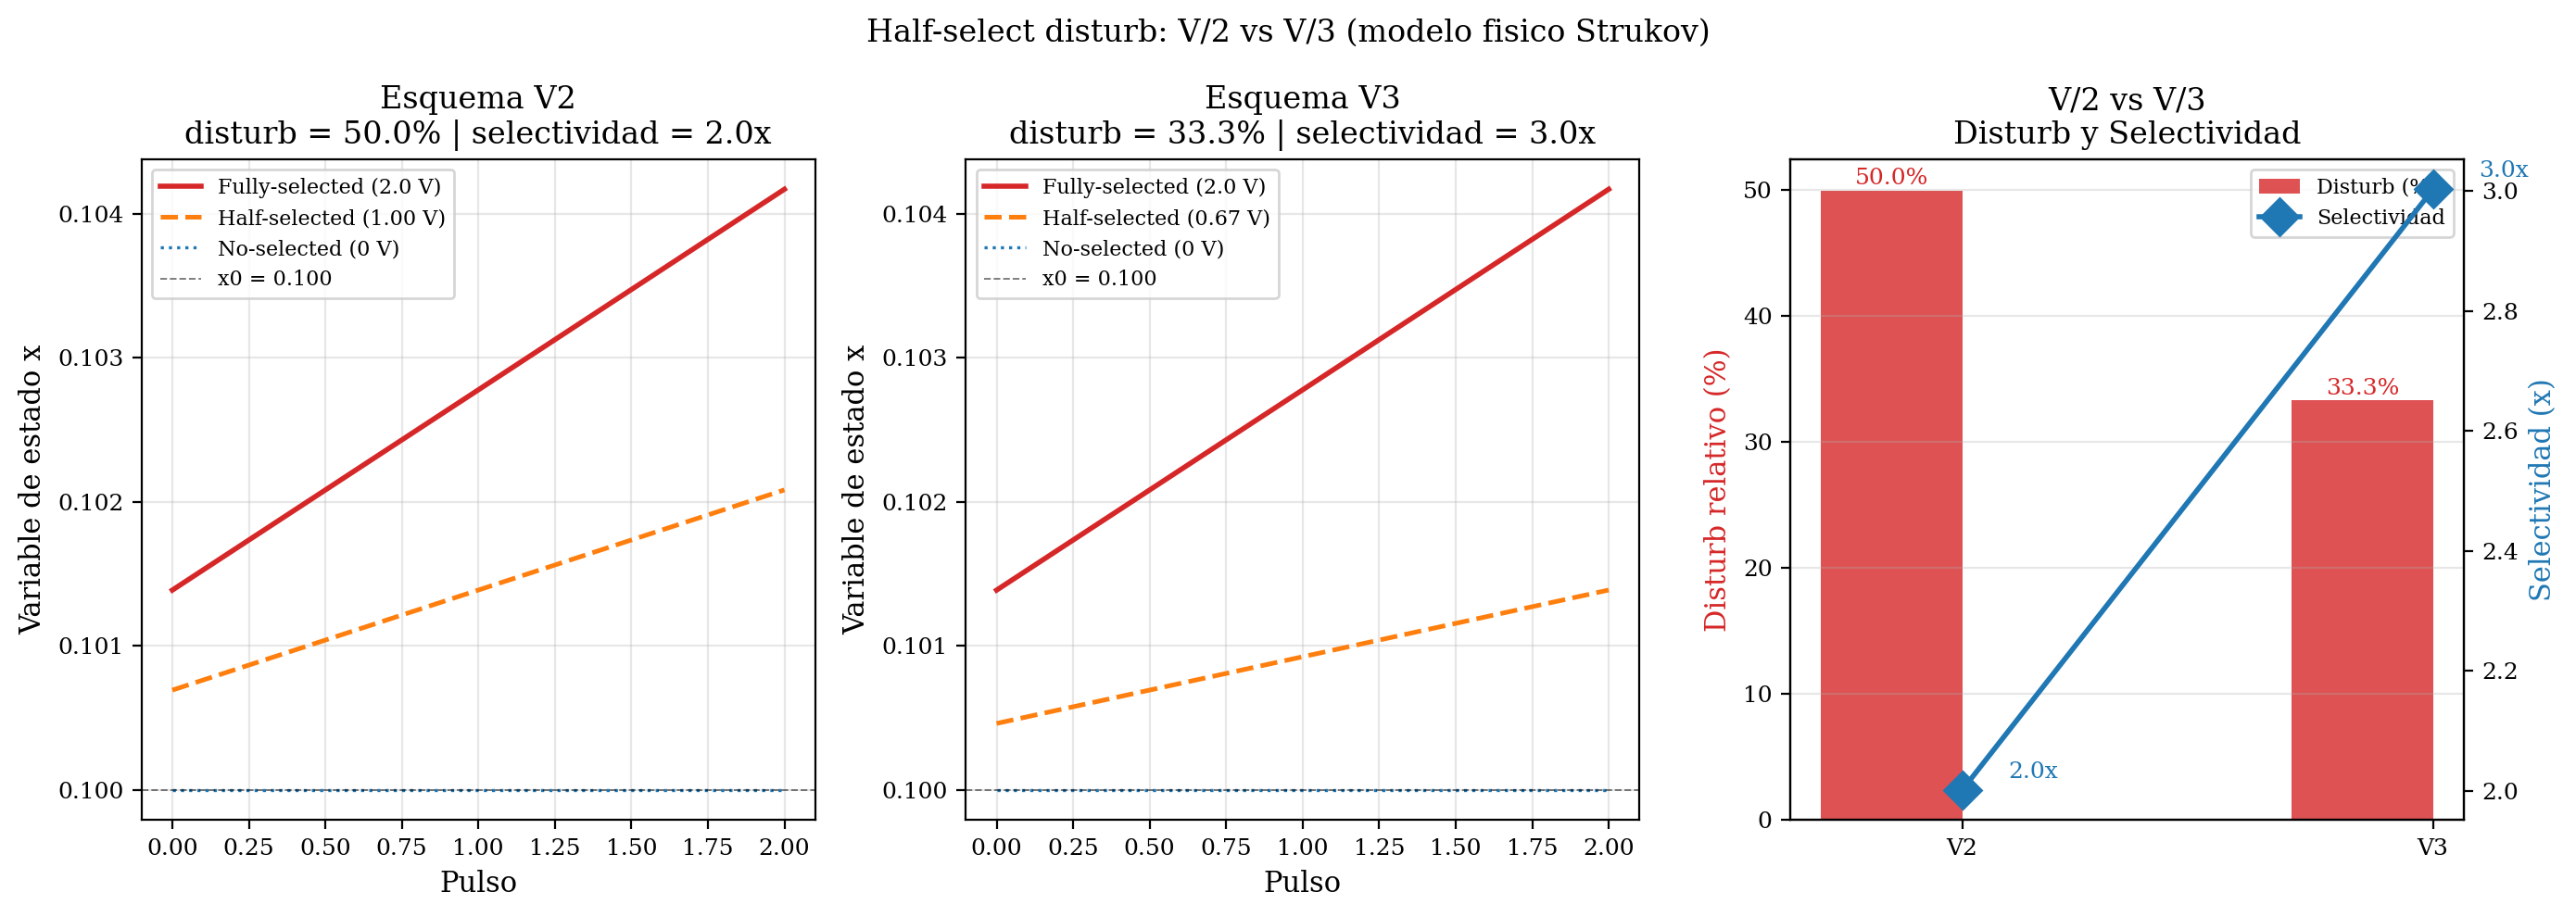
\includegraphics[width=0.95\textwidth]{experiments/figures/exp05_v2_vs_v3.png}
  \caption{Evolución de $X$ para celda fully-, half- y no-selected bajo 3 pulsos.}
  \label{fig:exp05}
\end{figure}

\paragraph{Exp.~6 --- Estado en reposo del modelo}
El resultado reportado tras 1000 pasos con $V_{\text{rows}}=0\,\text{V}$ es un cambio máximo en $X$ de $\Delta_{\max}=0$ bajo las condiciones del experimento. Esto describe el modelo y protocolo evaluados, no certifica la retención de un dispositivo físico.
\begin{figure}[H]
  \centering
  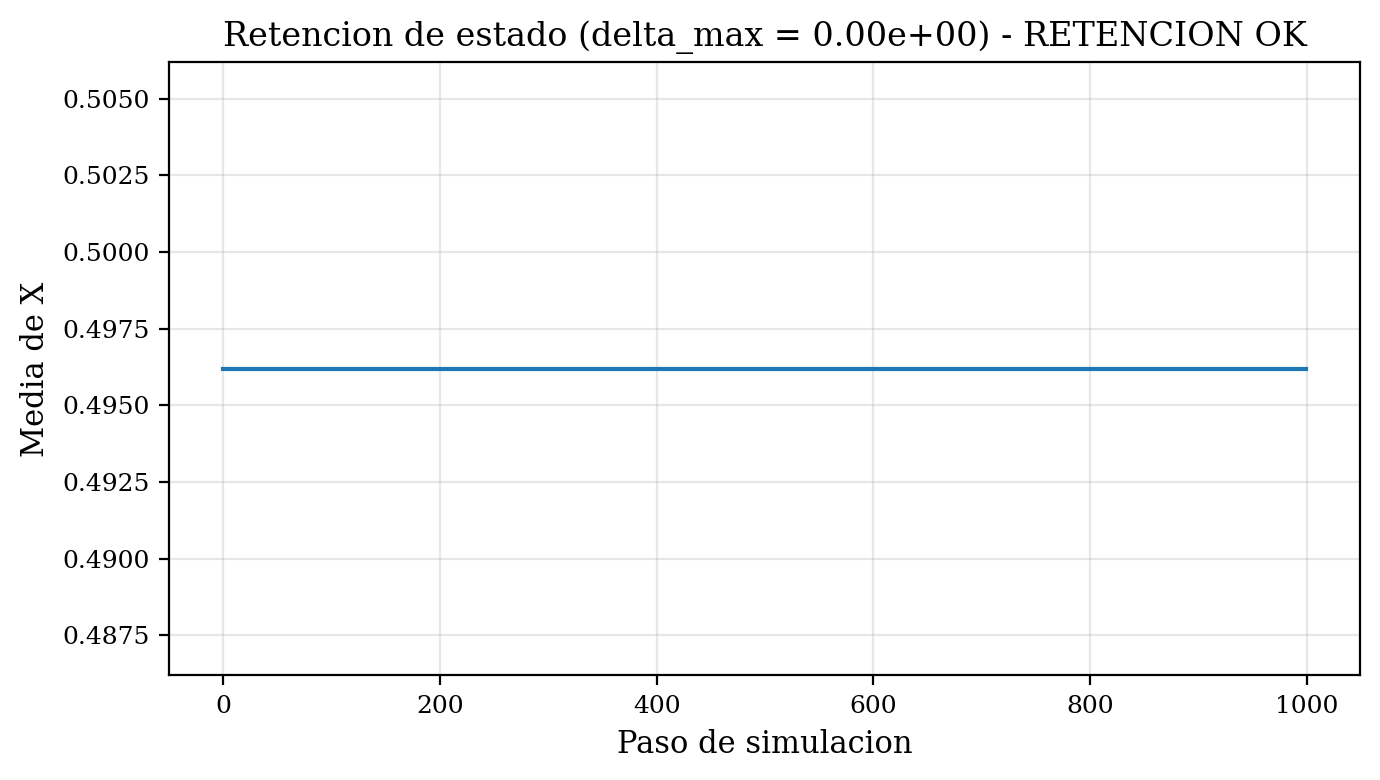
\includegraphics[width=0.62\textwidth]{experiments/figures/exp06_retention.png}
  \caption{Media de $X$ durante 1000 pasos en reposo para la simulación reportada.}
  \label{fig:exp06}
\end{figure}

\paragraph{Exp.~7 --- Respuesta simulada a pulsos LTP/LTD}
La Figura~\ref{fig:exp07} muestra la respuesta reportada del modelo bajo pulsos de potenciación (LTP, $+1\,\text{V}$) y depresión (LTD, $-1\,\text{V}$). Para 50 pulsos desde $x_0=0.1$, se reportan $x=0.135$ para LTP y $x=0.066$ para LTD. Estos valores describen la ejecución simulada y no se presentan como una respuesta experimental de un dispositivo real.
\begin{figure}[htbp]
  \centering
  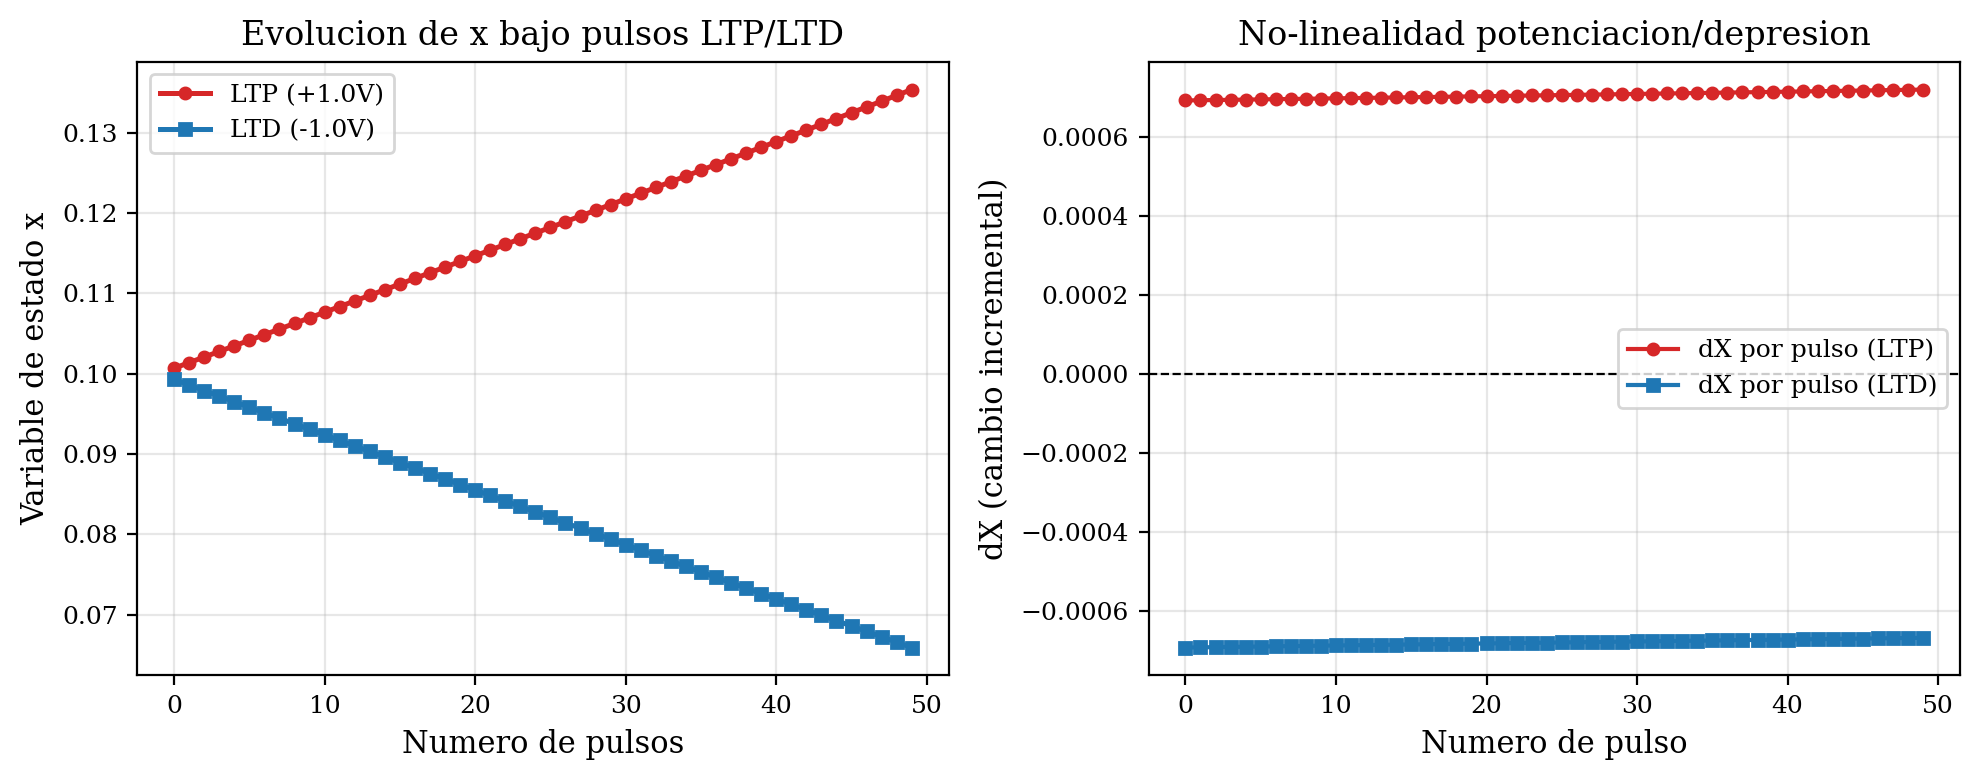
\includegraphics[width=0.88\textwidth]{experiments/figures/exp07_ltp_ltd.png}
  \caption{LTP/LTD y derivada discreta. La no-linealidad satura suavemente los extremos.}
  \label{fig:exp07}
\end{figure}

\paragraph{Exp.~8 --- Variabilidad dispositivo a dispositivo (D2D)}
La Figura~\ref{fig:exp08} cuantifica la dispersión de $I_{\text{col}}$ entre 20 crossbars virtuales. La variabilidad dispositivo-a-dispositivo se caracteriza por $CV(I_{\text{col}}) = 40.3\%$ en términos de la corriente integrada, equivalente al $4.0\%$ del rango dinámico de $\mathbf{G}$.
\begin{figure}[H]
  \centering
  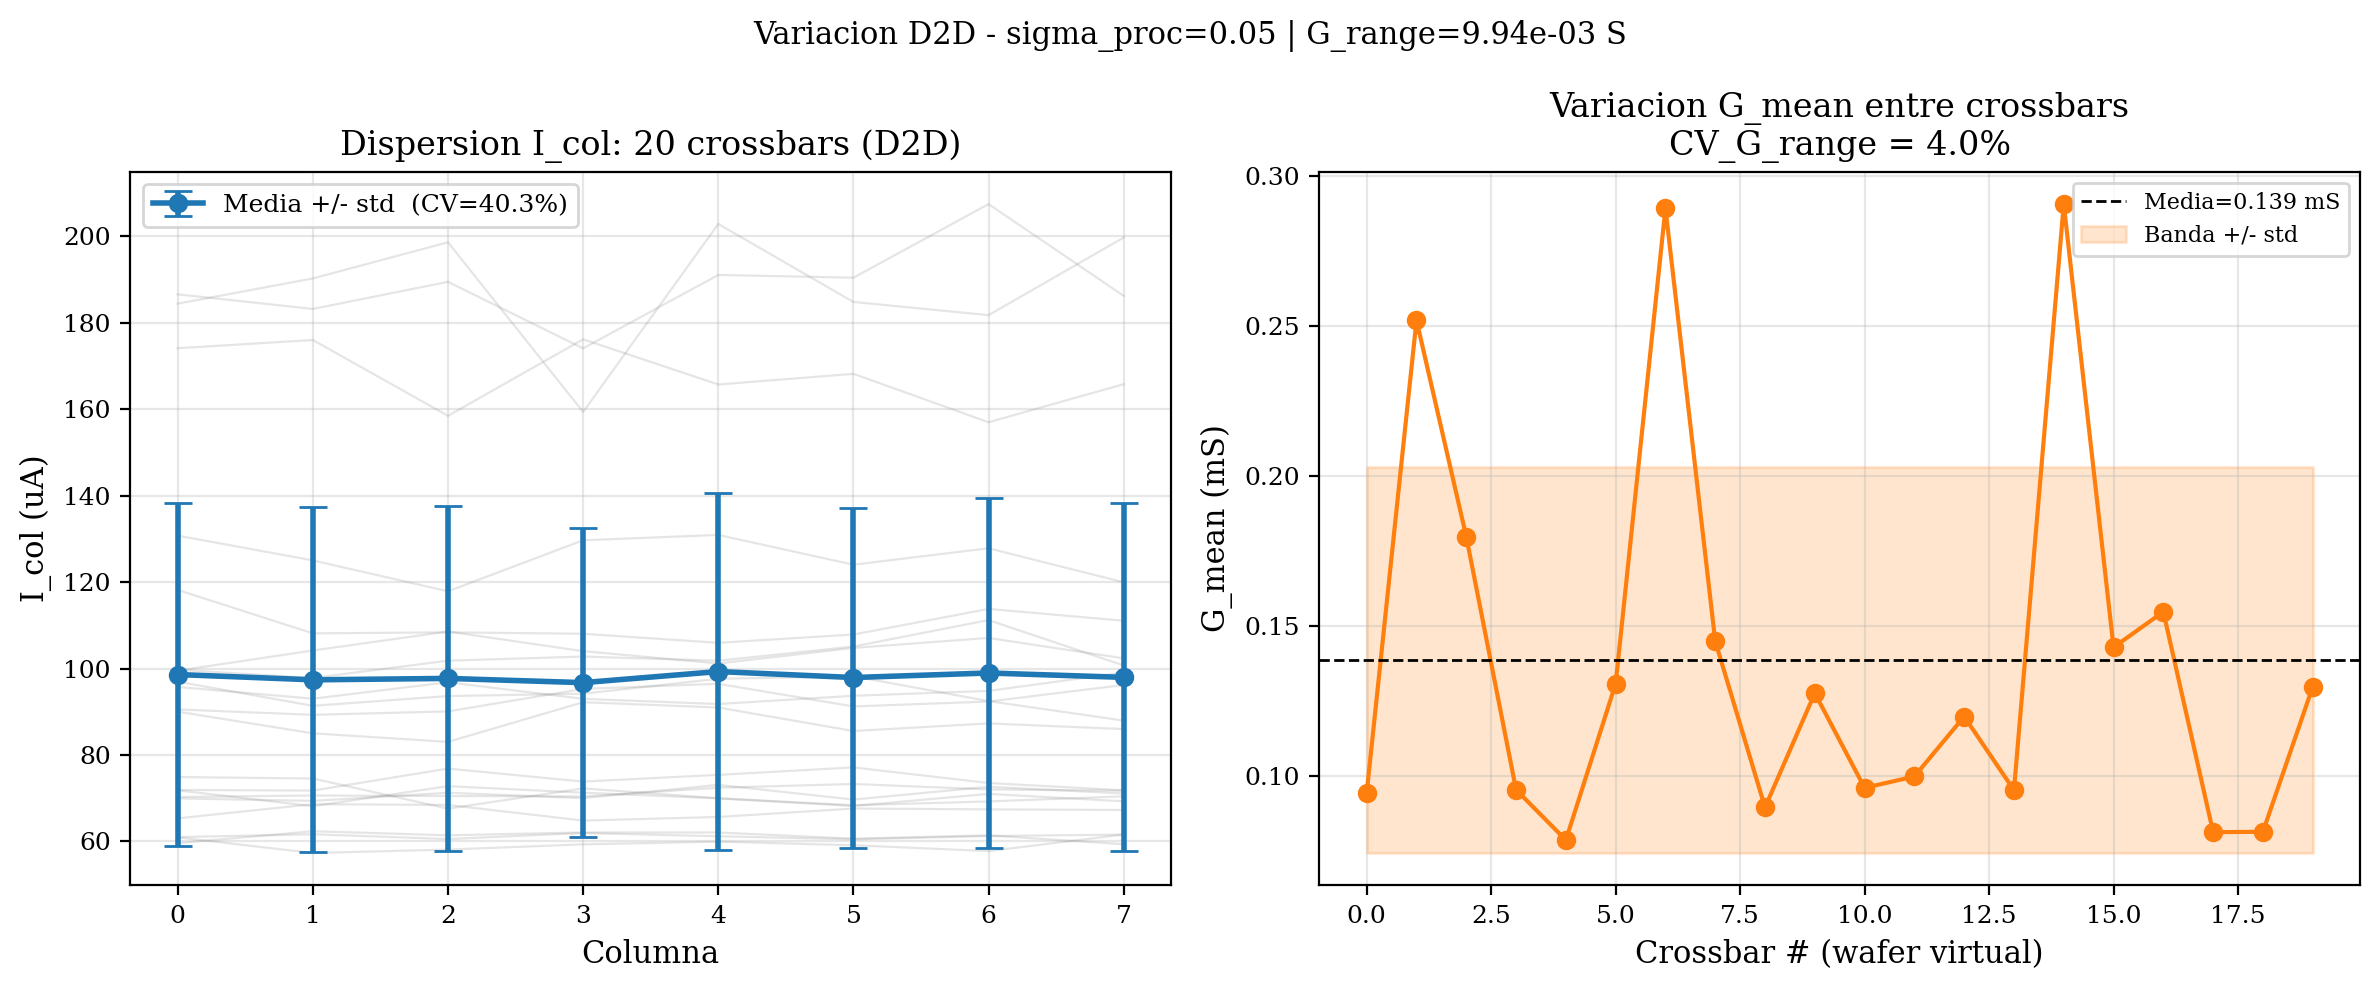
\includegraphics[width=0.88\textwidth]{experiments/figures/exp08_d2d_reproducibility.png}
  \caption{Dispersión de $I_{\text{col}}$ y variación de $\bar{G}_{\text{mean}}$ entre 20 crossbars virtuales.}
  \label{fig:exp08}
\end{figure}

\paragraph{Exp.~9 --- Costo computacional del solver MNA}
La Figura~\ref{fig:exp09} presenta un ajuste empírico reportado de
$\mathcal{O}(N^{0.85})$ y un tiempo aproximado de $\sim 3$ ms por paso para
$N=24$ en el equipo usado entonces. El exponente es propio de esa muestra y
configuración: no establece la complejidad asintótica del solver ni permite
generalizar la comparación con $\mathcal{O}(N^3)$ sin conocer el rango medido,
el hardware y el procedimiento de temporización.
\begin{figure}[H]
  \centering
  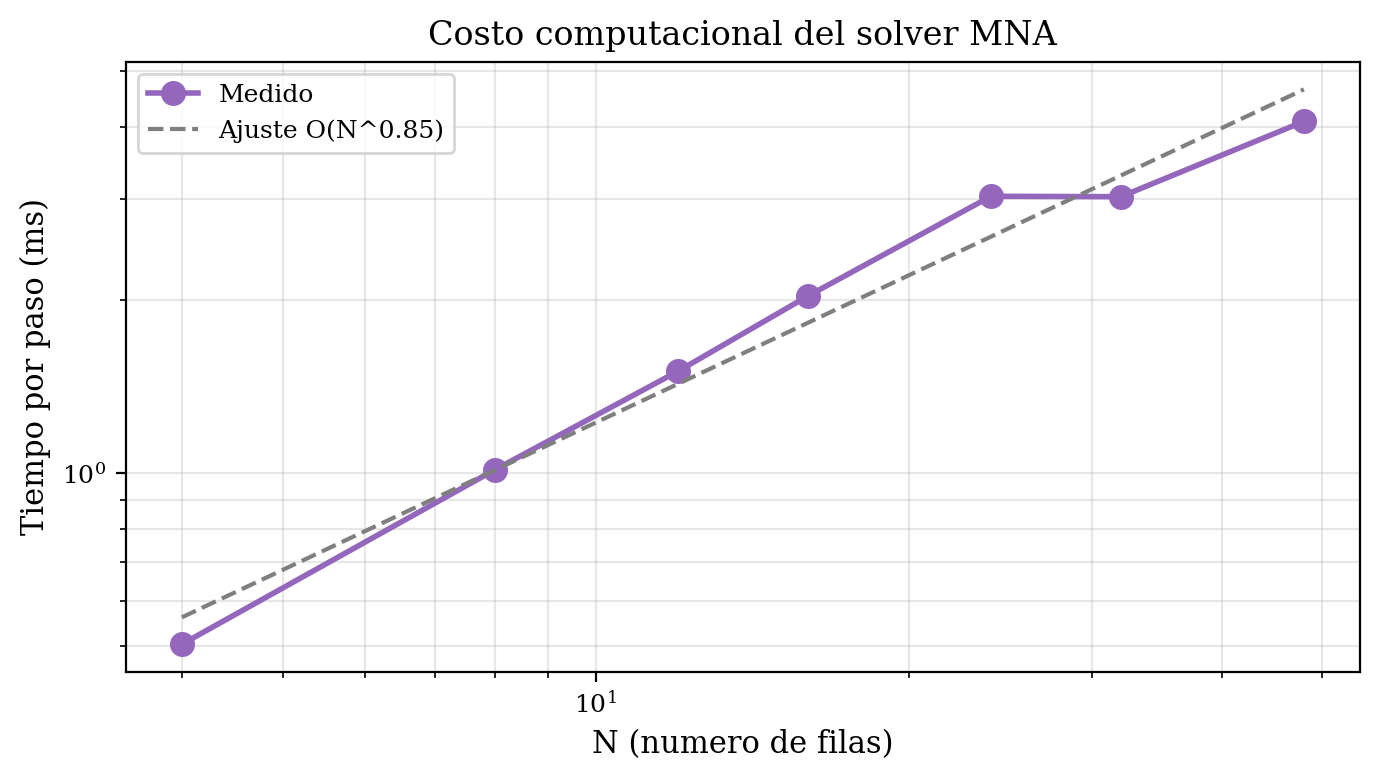
\includegraphics[width=0.62\textwidth]{experiments/figures/exp09_computational_cost.png}
  \caption{Costo computacional reportado del solver MNA en función de $N$.
El ajuste de las muestras archivadas es $\mathcal{O}(N^{0.85})$.}
  \label{fig:exp09}
\end{figure}

\paragraph{Exp.~10 --- Crosstalk entre columnas}
La Figura~\ref{fig:exp10} expone el efecto de crosstalk: al excitar únicamente la fila 0, las otras columnas muestran una desviación media del $13.32\%$ por interacción parásita MNA.
\begin{figure}[H]
  \centering
  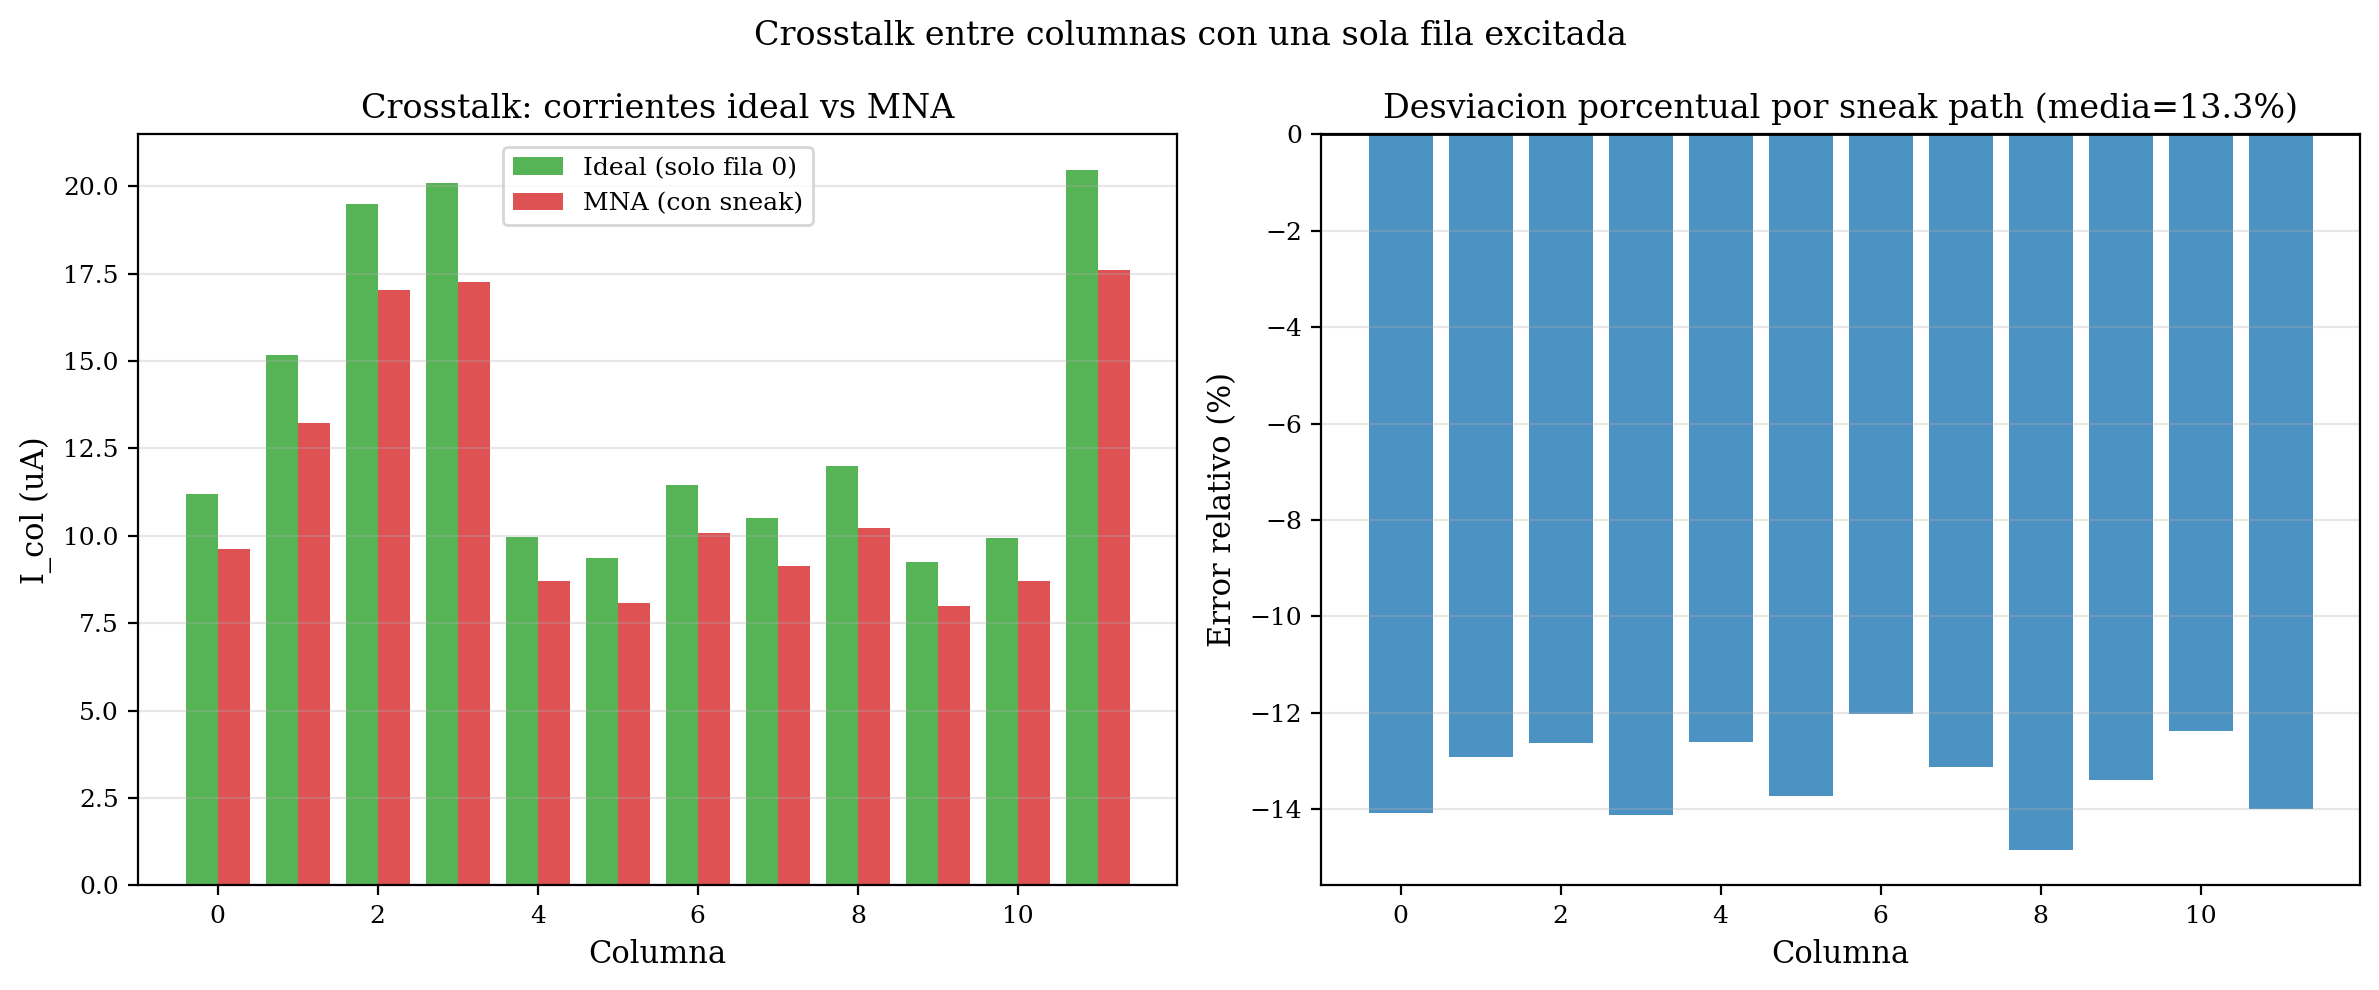
\includegraphics[width=0.88\textwidth]{experiments/figures/exp10_crosstalk.png}
  \caption{$I_{\text{col}}$ real vs.\ ideal al excitar únicamente la fila 0.}
  \label{fig:exp10}
\end{figure}

\paragraph{Alcance de los resultados de la Etapa 4}
Los diez experimentos anteriores y las figuras del agente documentan
resultados guardados de simulaciones, no mediciones de hardware. Para evitar
repetir sus cifras en un segundo resumen, esta sección deja cada resultado
junto a su configuración y figura; la tabla maestra del Apéndice C resume
únicamente las verificaciones V01--V28.
